%%%%%%%%%%%%%%%%%%%%%%%%%%%%%%%%%%%%%%%%%%%%%%%%%%%%%%%%%%%%%%%%%%%%%%%%%%%%%%%%%%%%%%%%%%%%%%%%%%%
% Chapter 4 -> Experiments
% Author: Eduardo G Gusmao
%%%%%%%%%%%%%%%%%%%%%%%%%%%%%%%%%%%%%%%%%%%%%%%%%%%%%%%%%%%%%%%%%%%%%%%%%%%%%%%%%%%%%%%%%%%%%%%%%%%
\chapter{Experiments}
\label{cha:experiments}

\graphicspath{{chapter4/figs/}}

The main goal of this chapter is to present the experimental framework used in this thesis. In this chapter we are going to:
\begin{itemize}
\item Describe the execution of our novel computational footprinting approach HINT, which was formally presented in the previous chapter.
\item Describe the execution of all competing computational footprinting methods.
\item Formalize the computational footprinting method evaluation methodologies and metrics.
\item Introduce common downstream analyses, which use footprint predictions to make inferences about the regulatory network of a cell.
\item State all statistical methods employed in this thesis.
\end{itemize}

% Introduction 1
The experimental framework used in this thesis is divided in two parts: the execution and the evaluation of computational footprinting methods. First, we describe the execution of computational footprinting methods (Section~\ref{sec:execution.computational.footprinting.methods}). We provide the detailed experimental workflow of our computational footprinting method HINT. Furthermore, we describe the execution of all competing methods used in this thesis. In the second part, we define the methodology used to evaluate all computational footprinting methods (Section~\ref{sec:evaluation.computational.footprinting.methods}). We describe two different evaluation strategies: the traditional transcription factor (TF) ChIP-seq approach and the novel strategy we devised, which is based on gene expression.

% Introduction 2
In addition, we describe two common downstream analyses, which use footprint predictions: the TF enrichment analysis and the \emph{de novo} motif finding. These analyses are described in Section~\ref{sec:footprint.downstream.analyses}. Moreover, all statistical methods used on the analyses presented in this thesis are described in Section~\ref{sec:further.statistical.methods}. Finally, we close this chapter with a final discussion on our experimental framework (Section~\ref{sec:discussion.4}).

%%%%%%%%%%%%%%%%%%%%%%%%%%%%%%%%%%%%%%%%%%%%%%%%%%%%%%%%%%%%%%%%%%%%%
% Section: Execution of Computational Footprinting Methods
%%%%%%%%%%%%%%%%%%%%%%%%%%%%%%%%%%%%%%%%%%%%%%%%%%%%%%%%%%%%%%%%%%%%%
\section{Execution of Computational Footprinting Methods}
\label{sec:execution.computational.footprinting.methods}

% Introduction
In this section we describe the experimental framework regarding the execution of our computational footprinting method -- HINT -- and the competing footprinting methods (Figure~\ref{fig:gusmao_experiment_design_method}). First, we describe the data used as input for these methods: DNase-seq and histone modification ChIP-seq (Section~\ref{sec:execution.data}). Then, we proceed by characterizing HINT's signal processing pipeline (Section~\ref{sec:hint.signal.processing}) and HINT's execution (Section~\ref{sec:hint.method.execution}). Finally, we describe the execution of all competing computational footprinting methods (Section~\ref{sec:competing.methods})

% Figure - Experimental framework of the execution of the computational footprinting methods
\begin{figure}[h!]
\centering
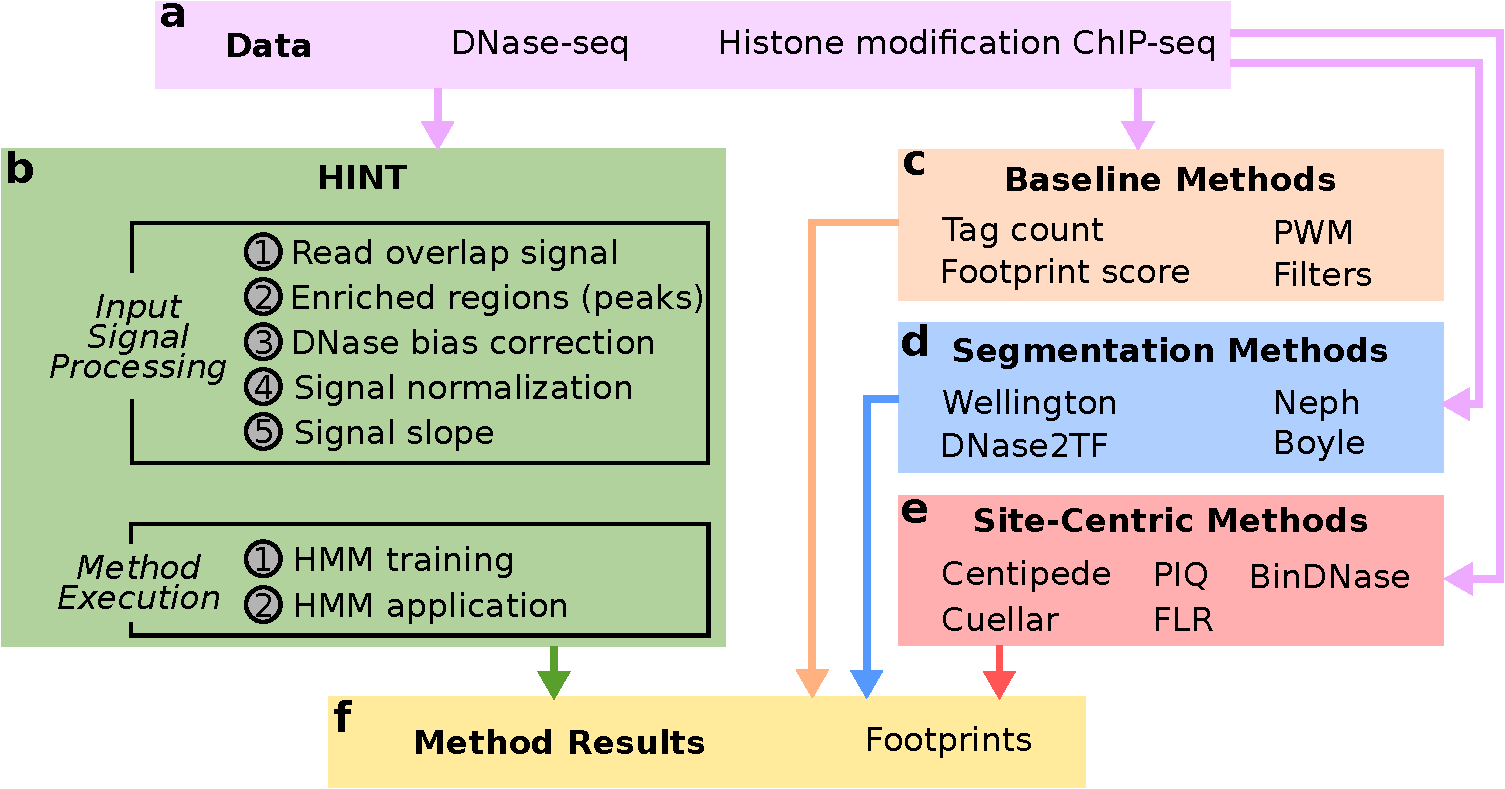
\includegraphics[width=0.9\textwidth]{gusmao_experiment_design_method}
\caption[Experimental framework of the execution of the computational footprinting methods]{\textbf{Experimental framework of the execution of the computational footprinting methods.} (\textbf{a}) The computational footprinting methods take as input different combinations of DNase-seq and histone modification ChIP-seq data. (\textbf{b}) The computational footprinting method proposed in this thesis -- HINT -- is divided in: input signal processing and method execution. (\textbf{c}--\textbf{e}) Competing methods, categorized as (\textbf{c}) baseline, (\textbf{d}) segmentation and (\textbf{e}) site-centric, are executed to perform a comparative analysis with the performance of HINT. (\textbf{f}) All computational footprinting methods generate footprint predictions.}
\label{fig:gusmao_experiment_design_method}
\end{figure}

%%%%%%%%%%%%%%%%%%%%%%%%%%%%%%%%%%%%%%%%%%%%%%%%%%%%%%%%%%%%%%%%%%%%%
% Section: Data
%%%%%%%%%%%%%%%%%%%%%%%%%%%%%%%%%%%%%%%%%%%%%%%%%%%%%%%%%%%%%%%%%%%%%
\subsection{Data}
\label{sec:execution.data}

\subsubsection{Data-seq Data}

% DNase-seq
DNase-seq aligned reads were obtained in~\cite{encode2012}. We obtained data generated from the single-hit (labeled as ``SH'') and double-hit (labeled as ``DH'') DNase-seq protocols. Furthermore, we obtained naked deoxyribonucleic acid (DNA) DNase-seq data (labeled as ``NK''). The naked DNA DNase-seq data results from the application of the same DNase-seq protocol as shown for the single-hit and double-hit version (Section~\ref{sec:dnase.seq}); however it is applied to a cell in which all active TFs have been removed from the DNA. A full description on all DNase-seq data used in this thesis can be found at Supplementary Table~\ref{tab:dataencode.dnase}.

Each DNase-seq dataset correspond to the DNase-seq experiment aligned reads for one cell type. We divided the cell types in which we obtained DNase-seq data into three categories: \linebreak the {\tt Comparative Dataset}, {\tt Analysis Dataset} and {\tt Full Dataset}. Below, we show the cell types associated to each category:

% DNase-seq cell types
\begin{itemize}
\item {\tt Comparative Dataset} -- Data used in the method comparison analysis:
\begin{itemize}
\item Single-hit DNase-seq protocol (SH): H1-hESC, K562 and GM12878.
\end{itemize}
\item {\tt Analysis Dataset} -- Data used in the analysis of relevant computational footprinting features:
\begin{itemize}
\item Single-hit DNase-seq protocol (SH): H1-hESC, HeLa-S3, HepG2, HUVEC, K562, \linebreak GM12878, LNCaP and MCF-7.
\item Double-hit DNase-seq protocol (DH): H7-hESC, HepG2, HUVEC, K562 and m3134.
\item Naked DNA DNase-seq protocol (NK): MCF-7, K562 and IMR90.
\end{itemize}
\item {\tt Full Dataset} -- All cell types from the encyclopedia of DNA elements (ENCODE) Tier 1 and Tier 2 experiments (SH, DH and NK)~\citep{encode2012}. These data were used to investigate relevant features regarding the DNase-seq sequence cleavage bias.
\end{itemize}

\subsubsection{Histone Modification ChIP-seq Data}

% Histone modifications ChIP-seq
Histone modifications ChIP-seq aligned reads were also obtained in~\cite{encode2012}. We only obtained histone modification ChIP-seq data from cell types of the {\tt Comparative Dataset}, i.e. H1-hESC, K562 and GM12878. For each cell type, it was obtained data regarding the activating histone modifications: H3K4me1, H3K4me3, H3K9ac, H3K27ac and H2A.Z. Additionally, to perform some analysis of relevant computational footprinting features we obtained data regarding the histone modifications H3K4me1 and H3K4me3 for cell types HeLa-S3 and HepG2. See Supplementary Table~\ref{tab:dataencode.histone} for a full histone modification ChIP-seq data description.

\subsubsection{Genomic Information on Experimental Datasets}

% Additional data information
Both DNase-seq and histone modification ChIP-seq data are based on the human genome build 37 (hg19), except the DNase-seq for m3134 cell type, which is based on mouse genome build 37 (mm9). Chromosome~Y was removed from all analyses. It is usual to remove chromosome Y from such types of analyses since it is present in male subjects only; and therefore introduces biases. The genomic sequences (DNA) for the human genome (hg19) and mouse genome (mm9) were also obtained in~\cite{encode2012}.

%%%%%%%%%%%%%%%%%%%%%%%%%%%%%%%%%%%%%%%%%%%%%%%%%%%%%%%%%%%%%%%%%%%%%
% Section: HINT Signal Processing
%%%%%%%%%%%%%%%%%%%%%%%%%%%%%%%%%%%%%%%%%%%%%%%%%%%%%%%%%%%%%%%%%%%%%
\subsection{HINT Signal Processing}
\label{sec:hint.signal.processing}

% Introduction
HINT takes as input DNase-seq and/or histone modification ChIP-seq data. Here we discuss the processing steps of such data from the obtained aligned reads to the final signal which is used by HINT to make the footprint predictions. For simplicity, we ignore the fact that signals and intervals are defined on distinct chromosomes.

%%%%%%%%%%%%%%%%%%%%%%%%%%%%%%%%%%%%%%%%%%%%%%%%%%%%%%%%%%%%%%%%%%%%%
% Section: Read Overlap Signal
%%%%%%%%%%%%%%%%%%%%%%%%%%%%%%%%%%%%%%%%%%%%%%%%%%%%%%%%%%%%%%%%%%%%%
\subsubsection{Read Overlap Signal}

% Genomic signal creation
We obtained the DNase-seq aligned reads and histone modification ChIP-seq aligned reads in~\cite{encode2012} (Section~\ref{sec:execution.data}). These datasets are already processed to remove known experimental and computational artifacts~\citep{encode2012,derrien2012,ashoor2013,diaz2012}. We created the read overlap signal from both DNase-seq and histone modification ChIP-seq pre-processed aligned reads as described in Section~\ref{sec:read.overlap.signal}.

%%%%%%%%%%%%%%%%%%%%%%%%%%%%%%%%%%%%%%%%%%%%%%%%%%%%%%%%%%%%%%%%%%%%%
% Section: DNase Hypersensitivity Sites and Histone Modification ChIP-seq Peaks
%%%%%%%%%%%%%%%%%%%%%%%%%%%%%%%%%%%%%%%%%%%%%%%%%%%%%%%%%%%%%%%%%%%%%
\subsubsection{DNase Hypersensitivity Sites and Histone Modification ChIP-seq Peaks}

% Introduction
To optimize execution time we constraint the application of our method (HINT) only in genomic regions enriched with either DNase-seq and histone modification ChIP-seq signals. Enriched regions are genomic regions with more reads aligned than expected by chance, given a statistical model. Here, we describe how we obtained the enriched regions for DNase-seq data -- called DNase hypersensitivity sites (DHSs) -- and the enriched regions for histone modification ChIP-seq data -- called histone modification ChIP-seq peaks.

% DNase Hypersensitivity Sites
\vspace{0.5cm}
\noindent
\emph{DNase Hypersensitivity Sites (DHSs)}
\vspace{0.3cm}

% DHS estimation
\noindent
DHSs, i.e. regions enriched with DNase-seq data, are estimated based on the DNase-seq read overlap signal. The process consists on evaluating a smoothed DNase-seq signal and then finding regions with more aligned reads than expected by chance based on a $p$-value cutoff of $0.01$ calculated based on a fitted Gamma distribution. The Gamma distribution was shown to outperform other models for DNase-seq data~\citep{boyle2008b}.

% F-seq
For that, we used the F-seq software~\citep{boyle2008b}, which was devised specially for DNase-seq data and has shown to provide accurate DHSs~\citep{boyle2008b,boyle2011}. We run the F-seq software version 1.81 with the default parameters, except for the feature length option (set to $300$)~\citep{boyle2011}. F-seq source code is found in \url{http://fureylab.web.unc.edu/software/fseq/}.

% Histone Modification ChIP-seq Peaks
\vspace{0.5cm}
\noindent
\emph{Histone Modification ChIP-seq Peaks}
\vspace{0.3cm}

% Introduction
\noindent
The histone modification ChIP-seq peaks were obtained by applying the ``model-based analysis for ChIP-seq'' (MACS) software~\citep{zhang2008} version 2.0.9 to the histone modification read overlap signals. Such peak-calling software was devised specially for ChIP-seq data. We executed MACS software with the default parameters. However, we used two extra command options which are indicated in the case of histone modification ChIP-seq (-{}-nomodel -{}-nolambda). The MACS software source code is found at \url{http://liulab.dfci.harvard.edu/MACS/}.

%%%%%%%%%%%%%%%%%%%%%%%%%%%%%%%%%%%%%%%%%%%%%%%%%%%%%%%%%%%%%%%%%%%%%
% Section: DNase-seq Sequence Cleavage Bias Correction
%%%%%%%%%%%%%%%%%%%%%%%%%%%%%%%%%%%%%%%%%%%%%%%%%%%%%%%%%%%%%%%%%%%%%
\subsubsection{DNase-seq Sequence Cleavage Bias Correction}

% Introduction
The intrinsic DNase-seq sequence cleavage bias was previously shown to affect certain footprinting methods~\citep{he2014}. In this study, we are going to explore the DNase-seq sequence cleavage bias correction using two approaches: (1) The ``DHS sequence bias'' considers the sequence bias estimates within DHSs of each DNase-seq experiment. This approach captures DNase I cleavage, read fragmentation and sequence complexity biases of DHSs of each DNase-seq experiment~\citep{he2014}. The ``naked DNA sequence bias'' considers the sequence bias estimates within naked DNA DNase-seq experiments~\citep{yardimci2014}. In this case, all DNA regions are open, therefore the sequence bias estimates will mainly capture the DNase I cleavage bias. Both strategies use the formalism described in Section~\ref{sec:dnaseseq.sequence.cleavage.bias}.

% DHS sequence bias
In the DHS sequence bias correction approach, we use the same DNase-seq dataset in which the read overlap genomic signal was created, to estimate the DNase-seq sequence cleavage bias. Furthermore, the genomic regions of interest $H$ from Section~\ref{sec:dnaseseq.sequence.cleavage.bias} correspond to the DHSs. In this case, each dataset (each DNase-seq experiment for a particular cell type) has their own DNase-seq sequence cleavage bias estimations and the correction is made on a cell-specific manner.

% Naked DNA sequence bias
In the naked DNA sequence bias correction approach, we use a naked DNA DNase-seq experiment to estimate the sequence cleavage bias. Moreover, the estimation is made on the whole genome, since there are no significantly enriched signals in such dataset. Therefore, the set of genomic regions of interest correspond to a single region which encompasses the whole genome, i.e. $H = \{ [1,n] \}$, where $n$ is the total number of base pairs (bp) in the genome. In this case, each naked DNA DNase-seq dataset has their own sequence cleavage bias estimations. The sequence cleavage bias correction for a DNase-seq dataset is made using the naked DNA DNase-seq sequence cleavage bias estimates which correlated best with the DHS sequence bias estimates for that DNase-seq dataset.

% k-mer
Another methodological choice is the size of the $k$-mer sequence cleavage bias estimates. For both approaches (DHS and naked DNA sequence bias correction) we used $6$-mers. As observed by~\cite{he2014}, a $6$-mer bias model captures significantly more information than $k < 6$ models and the information gained with $k > 6$ models are not significant and does not justify the increase in computational complexity (since the number of estimates is exponential).

%%%%%%%%%%%%%%%%%%%%%%%%%%%%%%%%%%%%%%%%%%%%%%%%%%%%%%%%%%%%%%%%%%%%%
% Section: Signal Normalization
%%%%%%%%%%%%%%%%%%%%%%%%%%%%%%%%%%%%%%%%%%%%%%%%%%%%%%%%%%%%%%%%%%%%%
\subsubsection{Signal Normalization}

% Introduction
In possession of the DNase-seq sequence cleavage bias corrected signals and read overlap histone modification ChIP-seq signals we proceed to the signal normalization step, which consists on the treatment of these genomic signals to: (1) reduce the within-dataset variability (as described in Section~\ref{sec:withindataset.normalization}) and (2) reduce the variability between these different genomic signals (as described in Section~\ref{sec:betweendataset.normalization}).

\vspace{0.5cm}
\noindent
\emph{Within-dataset Normalization}
\vspace{0.3cm}

% Within-dataset normalization
In the within-dataset normalization step we divide the genome in multiple bins, to estimate and correct the magnitude of the signal peaks, as shown in Section~\ref{sec:withindataset.normalization}. The length of the bin, denoted by $\iota$ was set to $10,000$ bp. The reason for such a choice is that shorter regions would not capture enough signal and lose statistical power. On the other hand larger regions would not achieve the goal of correcting the magnitude of the peaks within the dataset range of signals~\citep{gusmao2014}.

\vspace{0.5cm}
\noindent
\emph{Between-dataset Normalization}
\vspace{0.3cm}

% Between-dataset normalization
In the between-dataset normalization step, we fit the signal into a logistic function to force the values to be within the interval $[0,1]$. In this step, we estimated the mean $\mu$, standard deviation $\sigma$ and the percentile $\varsigma$ using data from chromosome~1, which was removed from the evaluation strategy. Furthermore, we used the $98^\text{th}$ percentile. Such a choice was made by observing the amount of the genome which is enriched for both DNase-seq and histone modification ChIP-seq, which is, on average \approxy$2\%$~\citep{gusmao2014}.

%%%%%%%%%%%%%%%%%%%%%%%%%%%%%%%%%%%%%%%%%%%%%%%%%%%%%%%%%%%%%%%%%%%%%
% Section: Signal Slope
%%%%%%%%%%%%%%%%%%%%%%%%%%%%%%%%%%%%%%%%%%%%%%%%%%%%%%%%%%%%%%%%%%%%%
\subsubsection{Signal Slope}

% Introduction
Given the normalized DNase-seq and histone modification ChIP-seq signals, we proceed to calculate the signals' slope. The goal is to create the additional slope signal required by HINT (as described in Section~\ref{sec:savitzkygolay.smoothing.slope}).

% Slope
In the application of the Savitzky-Golay technique to calculate the signals' slope, we used a $2^{\text{nd}}$-order polynomial. Furthermore, the odd-valued window size $\tau$ for smoothing and estimation of the slope of the signal was set to $9$ bp for the DNase-seq signal, as suggested by~\cite{boyle2011}. For the histone modification ChIP-seq signal, such parameter was set to $201$ bp, as it fits the read extension length ($\eta$) considered during the creation of the read overlap signal.

%%%%%%%%%%%%%%%%%%%%%%%%%%%%%%%%%%%%%%%%%%%%%%%%%%%%%%%%%%%%%%%%%%%%%
% Section: HINT Input Signal
%%%%%%%%%%%%%%%%%%%%%%%%%%%%%%%%%%%%%%%%%%%%%%%%%%%%%%%%%%%%%%%%%%%%%
\subsubsection{HINT Input Signal}

% Conclusion
After these processing steps we have four different input signals for our computational footprinting method HINT. Different HINT's hidden Markov model (HMM) topologies use different combinations of these four signals (the description of all topologies is found in Section~\ref{sec:hmm.topology}). The four HINT's input signals are:

\vspace{0.3cm}
\noindent
\textbf{1.} $\mathbf{x}^{\text{norm}}_{\text{dnase}}$ -- the real-valued vector of normalized DNase-seq genomic signals. \vspace{0.2cm} \\
\textbf{2.} $\mathbf{x}^{\text{slope}}_{\text{dnase}}$ -- the real-valued vector of slope DNase-seq genomic signals. \vspace{0.2cm} \\
\textbf{3.} $\mathbf{x}^{\text{norm}}_{\text{histone}}$ -- the real-valued vector of normalized histone modification ChIP-seq genomic signals. \vspace{0.2cm} \\
\textbf{4.} $\mathbf{x}^{\text{slope}}_{\text{histone}}$ -- the real-valued vector of slope histone modification ChIP-seq genomic signals. \\
\vspace{0.3cm}

% Example of normalized and slope signals
Figure~\ref{fig:gusmao_normslope} shows an example of two genomic regions with read overlap (count), normalized and slope signals for two distinct genomic regions. In this figure we are able to observe the effect of the within-dataset normalization strategy by looking at the different ranges of the histone modification base overlap count signal (in black) -- [$0$,$40$] on the genomic region depicted in Figure~\ref{fig:gusmao_normslope}a \emph{vs} [$0$,$80$] on the genomic region depicted in Figure~\ref{fig:gusmao_normslope}b in comparison to the range between these two regions of the normalized signal [$0$,$1$]. The normalization preserves the shape of the peaks and does not attenuate undesired background noise signals. Furthermore, the effect of the between-dataset normalization approach is more straightforward, as all normalized signals will be within the range [$0$,$1$]. Moreover, this figure shows the difference in resolution between the different data sources. While ChIP-seq peaks are smoothed and spans on average $250$ bp, the DNase-seq peaks can be as short as $5$ bp.

% Figure - Genomic signal processing examples
\begin{figure}[h!]
\centering
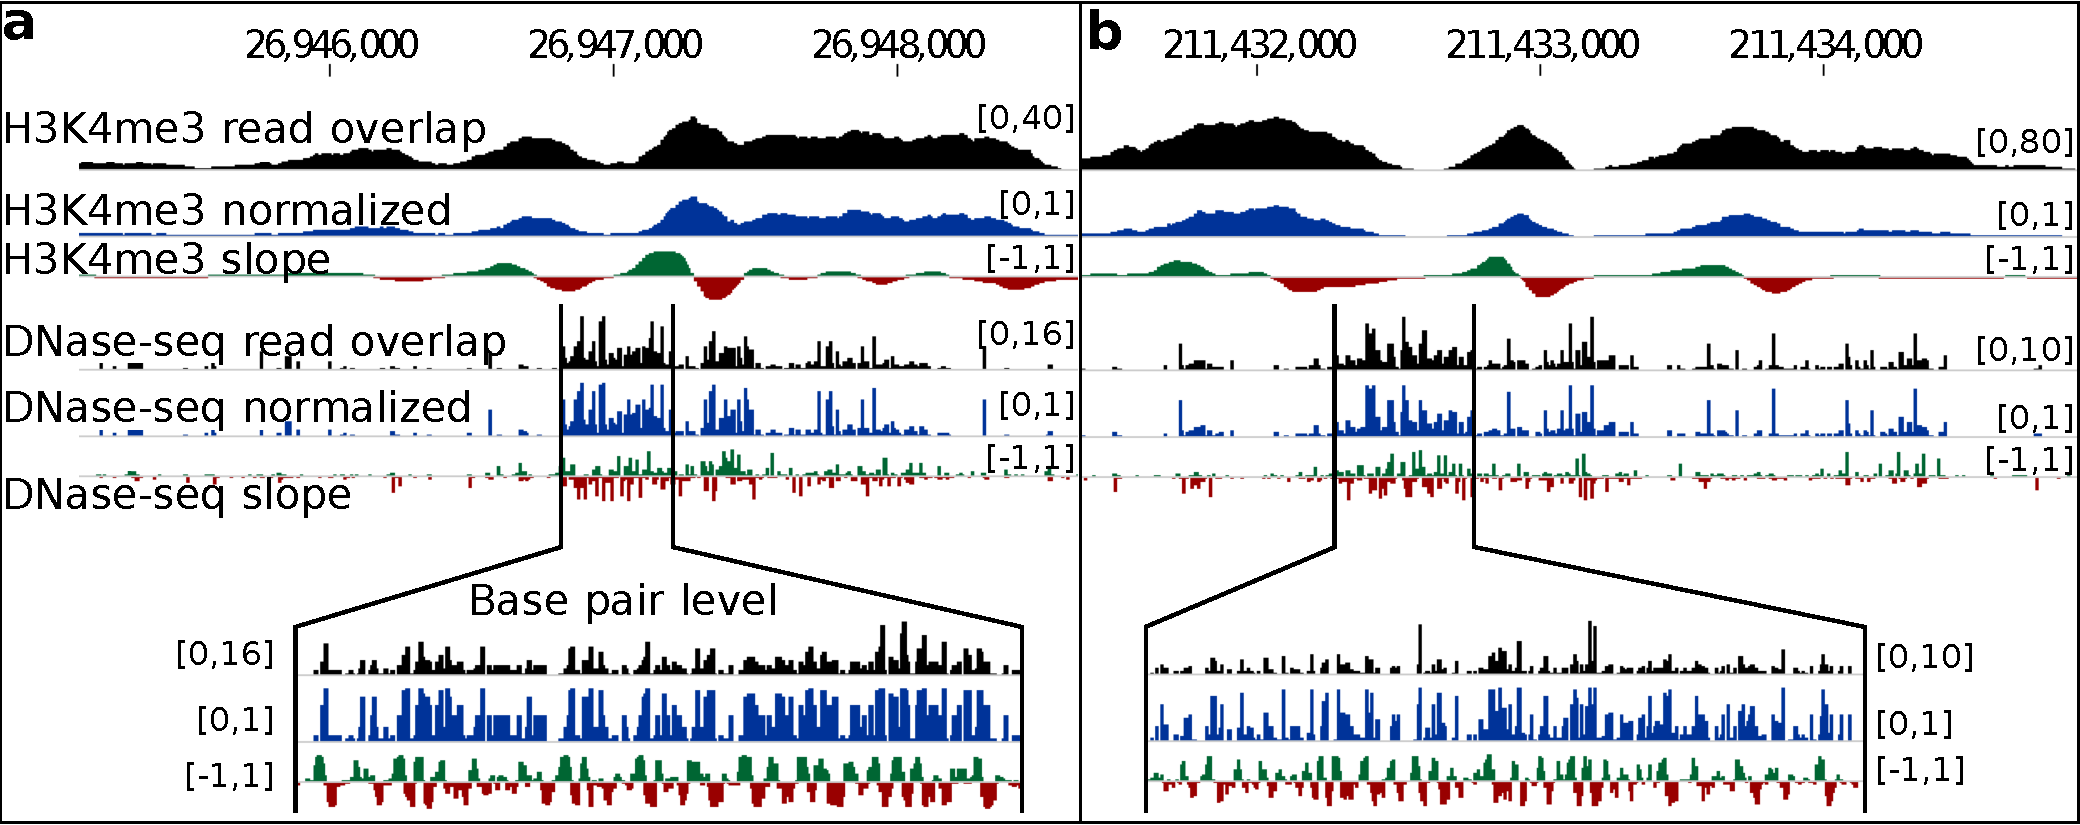
\includegraphics[width=0.99\textwidth]{gusmao_normslope}
\caption[Genomic signal processing examples]{\textbf{Genomic signal processing examples.} Examples of histone modification H3K4me3 ChIP-seq and DNase-seq signals before treatment (read overlap; in black), normalized (in blue) and after Savitzky-Goaly smoothing and differentiation (slope; positive values in green and negative values in red). Each signal's range is displayed between square brackets next to each signal. In this figure we show examples for two different regions in human chromosome~1. \emph{Source:~\cite{gusmao2014}} (modified to fit thesis format and/or clarify key points).}
\label{fig:gusmao_normslope}
\end{figure}

%%%%%%%%%%%%%%%%%%%%%%%%%%%%%%%%%%%%%%%%%%%%%%%%%%%%%%%%%%%%%%%%%%%%%
% Section: HINT Method Execution
%%%%%%%%%%%%%%%%%%%%%%%%%%%%%%%%%%%%%%%%%%%%%%%%%%%%%%%%%%%%%%%%%%%%%
\subsection{HINT Method Execution}
\label{sec:hint.method.execution}

% Introduction
Our computational footprinting method HINT segments the genome using normalized and slope versions of the DNase-seq and histone modification ChIP-seq signals. Such segmentation task is performed on the basis of the grammar of active transcription factor binding sites (TFBSs). As shown in Section~\ref{sec:hmm.topology} we have devised a number of different HMM topologies, which take different combinations of input signals and address particularities of the TFBS patterns on the open chromatin data. Here, we provide experimental details on how HINT is trained and applied on the genome.

%%%%%%%%%%%%%%%%%%%%%%%%%%%%%%%%%%%%%%%%%%%%%%%%%%%%%%%%%%%%%%%%%%%%%
% Section: HINT Training
%%%%%%%%%%%%%%%%%%%%%%%%%%%%%%%%%%%%%%%%%%%%%%%%%%%%%%%%%%%%%%%%%%%%%
\subsubsection{HINT Training}

% Manual annotation - introduction
We train the HMM models in a supervised manner. Briefly, a manual annotation is created for each cell type, histone modification and HMM topology (Figures~\ref{fig:gusmao_hmm_footprinting}--~\ref{fig:gusmao_model5}) based on the DNase-seq and histone modification ChIP-seq data.

% Manual annotation - region selection
We selected a $10,000$ bp region (with genomic coordinates $211,428,000$--$211,438,000$ in human chromosome~1) around the promoter region of the gene RCOR3 and performed a cell-specific manual annotation, in which each genomic position is assigned with a state from our HMM topology. This promoter-proximal regulatory region annotated with HMM states was used to train the models which use histone modifications H3K4me3, H3K9ac, H3K27ac and H2A.Z. As the histone modification H3K4me1 is known to be associated to distal regulatory regions, we have additionally annotated an enhancer region (with genomic coordinates $26,942,000$--$26,952,000$ in human chromosome~1). The selection of these regions was made randomly, but we checked~\cite{encode2012} tracks for evidence that the gene RCOR3 was expressed in all cell types analyzed and that the enhancer region was far ($>100$ Kbp) from known genes and expressed regions but associated with the expression of the closest gene's transcription start site (TSS).

% Manual annotation - process + training
In order to help the annotation of the footprints, motif-predicted binding sites (MPBSs) obtained by applying motif matching with all position frequency matrices (PFMs) from Jaspar~\citep{mathelier2014}, Uniprobe~\citep{robasky2011} and Transfac~\citep{matys2006} PFM repositories were detected inside the training regions (the details on the identification of MPBSs can be found in Section~\ref{sec:motif.predicted.binding.sites}). We consider ``real'' footprints all the DNase-seq signal depleted regions between two DNase-seq peaks that overlap a MPBS. For the \textsc{histone-only model}, we considered as footprints all the DHSs within these regions. We trained five HMMs per cell type, one for each histone modification (H3K4me3, H3K9ac, H3K29ac and H2A.Z with the promoter-proximal regulatory region and H3K4me1 with the distal regulatory region). In the case of the \textsc{DNase-only model}, only one HMM was trained for each cell type. Such training was performed in the promoter-proximal region. The regions used for training were excluded from all further analyses. In possession of the manually annotated regions for each cell type, histone modification and HMM topology, all HMMs were trained using the maximum-likelihood process described in Section~\ref{sec:hmm.training}.

% Example of HMM parameters - transition
Here, we show an example of a complete set of HMM parameters, regarding the \textsc{original DNase + histone} HMM topology (Figure~\ref{fig:gusmao_hmm_footprinting}) trained with DNase-seq $+$ H3K4me3 using data from the H1-hESC cell. The Table~\ref{tab:hmmtrans} represents the transition matrix. Each number represents the probability of performing a transition from the HMM state depicted in the table's first row to the HMM state depicted in the table's first column. In this transition matrix we are able to observe that only the self-transitions and the transitions allowed by our model topology have a non-zero probability. The transition matrix is the structure that directly defines our HMM topology.

% Example of HMM parameters - emission mean
The Table~\ref{tab:hmmmean} exhibits the emission distribution mean values. It contains the mean in which each signal type (represented in the columns) assumes at each state (represented in the rows). A closer look into these vectors of means for each state and signal shows the grammar of active TFBS in a numerical form. The states {\tt BACK} and {\tt FOOTPRINT} have low absolute means for all signal types. {\tt UP}, {\tt TOP} and {\tt DOWN} states have, respectively, high positive, close to zero and low negative slope signals. Such emission parameters models the signal magnitude of the active TFBS grammar. We are able to model both magnitude and shape of the signals when we consider the transition probabilities and the mean component of the emission probability distributions.

% Example of HMM parameters - emission covariance matrix
Moreover, the Table~\ref{tab:hmmcov} shows all covariance matrices from the emission distributions. The full covariance matrix is depicted for each state, in which rows and columns are sorted by the input signals: DNase-seq normalized, DNase-seq slope, H3K4me3 normalized and H3K4me3 slope. The covariance matrix component of the emission probability distributions reflect the relationship between our signals in our multivariate model. For instance, it is interesting to observe a negative value ($-0.0053$) at the DNase level {\tt UP} state (UP(D) in the table) on the covariance matrix corresponding to the normalized DNase-seq \emph{vs} the normalized histone modification ChIP-seq signal. Such data behavior is in line with the observed grammar of TFBSs, where the DNase-seq signal generally start to increase at the decrease of the histone modification ChIP-seq signal. Finally, when we consider all HMM parameters, we are able to model the magnitude, shape and relationship between the chromatin dynamics signals.

% Example of HMM transition matrix
\begin{table}[t]
\footnotesize
\begin{center}
\caption[Example of HMM transition matrix]{\textbf{Example of HMM transition matrix.} Transition probabilities of the HMM trained with DNase $+$ H3K4me3 using H1-hESC data. Transitions are specified from the states in the rows to the states in the columns. Histone level states are denoted with ``(H)'' and DNase level states with ``(D)''. The {\tt FOOTPRINT} state is abbreviated as ``FP''. \emph{Source:~\cite{gusmao2014}} (modified to fit thesis format and/or clarify key points).}
\label{tab:hmmtrans}
    \renewcommand{\arraystretch}{1.2}
    \begin{tabular}{ lllllllll }
        \hline
        & \textbf{BACK} & \textbf{UP (H)} & \textbf{TOP (H)} & \textbf{DOWN (H)} & \textbf{UP (D)}
        & \textbf{TOP (D)} & \textbf{DOWN (D)} & \textbf{FP} \\
        \textbf{BACK}     & 0.9997 & 0.0003 & 0.0    & 0.0    & 0.0    & 0.0    & 0.0   & 0.0    \\
        \textbf{UP (H)}   & 0.0    & 0.9915 & 0.0085 & 0.0    & 0.0    & 0.0    & 0.0   & 0.0    \\
        \textbf{TOP (H)}  & 0.0    & 0.0    & 0.9901 & 0.0099 & 0.0    & 0.0    & 0.0   & 0.0    \\
        \textbf{DOWN (H)} & 0.0057 & 0.0    & 0.0    & 0.9861 & 0.0082 & 0.0    & 0.0   & 0.0    \\
        \textbf{UP (D)}   & 0.0    & 0.0    & 0.0    & 0.0    & 0.6515 & 0.3485 & 0.0   & 0.0    \\
        \textbf{TOP (D)}  & 0.0    & 0.0    & 0.0    & 0.0    & 0.0    & 0.783  & 0.217 & 0.0    \\
        \textbf{DOWN (D)} & 0.0    & 0.0339 & 0.0    & 0.0    & 0.0    & 0.0    & 0.577 & 0.3891 \\
        \textbf{FP}       & 0.0    & 0.0    & 0.0    & 0.0    & 0.0564 & 0.0    & 0.0   & 0.9436 \\
        \hline
    \end{tabular}
\end{center}
\end{table}

% Example of HMM emission's mean vectors
\begin{table}[t]
\footnotesize
\begin{center}
\caption[Example of HMM emission's mean vectors]{\textbf{Example of HMM emission's mean vectors.} Signals' mean values for each state of the HMM trained with DNase $+$ H3K4me3 using H1-hESC data. Histone level states are denoted with ``(H)'' and DNase level states with ``(D)''. The {\tt FOOTPRINT} state is abbreviated as ``FP''. \emph{Source:~\cite{gusmao2014}} (modified to fit thesis format and/or clarify key points).}
\label{tab:hmmmean}
    \renewcommand{\arraystretch}{1.2}
    \begin{tabular}{ lllll }
        \hline
        & \textbf{DNase norm.} & \textbf{DNase slope} & \textbf{Histone norm.} & \textbf{Histone slope} \\
        \textbf{BACK}     & 0.0045 & -0.0002 & 0.0441 & 0.0007  \\
        \textbf{UP (H)}   & 0.0501 & 0.0043  & 0.1983 & 0.2995  \\
        \textbf{TOP (H)}  & 0.0445 & -0.0075 & 0.4693 & 0.0158  \\
        \textbf{DOWN (H)} & 0.0636 & 0.0003  & 0.2309 & -0.4237 \\
        \textbf{UP (D)}   & 0.1537 & 0.6343  & 0.0894 & -0.0647 \\
        \textbf{TOP (D)}  & 0.4244 & 0.0059  & 0.1091 & -0.0735 \\
        \textbf{DOWN (D)} & 0.1578 & -0.6562 & 0.0816 & -0.0434 \\
        \textbf{FP}       & 0.0902 & -0.0162 & 0.1009 & -0.0436 \\
        \hline
    \end{tabular}
\end{center}
\end{table}



% Example of HMM emission's covariance matrices
\begin{table}[t]
\footnotesize
\begin{center}
\caption[Example of HMM emission's covariance matrices]{\textbf{Example of HMM emission's covariance matrices.} Covariance matrices for each state of the HMM trained with DNase $+$ H3K4me3 using H1-hESC data. Within each state's matrix, lines and rows are sorted by signal type as DNase-seq normalized, DNase-seq slope, H3K4me3 normalized and H3K4me3 slope. Histone level states are denoted with ``(H)'' and DNase level states with ``(D)''. The {\tt FOOTPRINT} state is abbreviated as ``FP''. \emph{Source:~\cite{gusmao2014}} (modified to fit thesis format and/or clarify key points).}
\label{tab:hmmcov}
    \renewcommand{\arraystretch}{1.2}
    \begin{tabular}{>{\centering\arraybackslash} m{0.2cm}
                    >{\centering\arraybackslash} m{1.2cm}
                    >{\centering\arraybackslash} m{1.2cm}
                    >{\centering\arraybackslash} m{1.2cm}
                    >{\centering\arraybackslash} m{1.2cm}|
                    >{\centering\arraybackslash} m{0.2cm}
                    >{\centering\arraybackslash} m{1.2cm}
                    >{\centering\arraybackslash} m{1.2cm}
                    >{\centering\arraybackslash} m{1.2cm}
                    >{\centering\arraybackslash} m{1.2cm} }
        \hline
        \multirow{4}{*}{\rotatebox[origin=c]{90}{\textbf{BACK}}}
        & 0.0025  & -0.0001 & 0.0001 & 0.0    &
        \multirow{4}{*}{\rotatebox[origin=c]{90}{\textbf{UP (H)}}}
        & 0.0222  & 0.0001  & 0.003  & 0.0057 \\
        & -0.0001 & 0.0025  & 0.0    & 0.0    &
        & 0.0001  & 0.0155  & 0.0006 & 0.0005 \\
        & 0.0001  & 0.0     & 0.0047 & 0.0    &
        & 0.003   & 0.0006  & 0.0101 & 0.0105 \\
        & 0.0     & 0.0     & 0.0    & 0.0019 &
        & 0.0057  & 0.0005  & 0.0105 & 0.0341 \\
        \hline
        \multirow{4}{*}{\rotatebox[origin=c]{90}{\textbf{TOP (H)}}}
        & 0.0216  & 0.0003  & -0.0009 & 0.0014  &
        \multirow{4}{*}{\rotatebox[origin=c]{90}{\textbf{DOWN (H)}}}
        & 0.0239  & 0.0001  & -0.0033 & -0.0002 \\
        & 0.0003  & 0.0196  & 0.0005  & 0.0003  &
        & 0.0001  & 0.009   & 0.0002  & -0.0006 \\
        & -0.0009 & 0.0005  & 0.0047  & -0.001  &
        & -0.0033 & 0.0002  & 0.0156  & -0.0095 \\
        & 0.0014  & 0.0003  & -0.001  & 0.0193  &
        & -0.0002 & -0.0006 & -0.0095 & 0.0313  \\
        \hline
        \multirow{4}{*}{\rotatebox[origin=c]{90}{\textbf{UP (D)}}}
        & 0.0705  & 0.0246  & -0.0053 & 0.0025  &
        \multirow{4}{*}{\rotatebox[origin=c]{90}{\textbf{TOP (D)}}}
        & 0.1559  & -0.002  & -0.0079 & 0.0052  \\
        & 0.0246  & 0.0714  & -0.0038 & -0.0015 &
        & -0.002  & 0.0384  & -0.0008 & 0.0021  \\
        & -0.0053 & -0.0038 & 0.0045  & -0.0056 &
        & -0.0079 & -0.0008 & 0.007   & -0.0096 \\
        & 0.0025  & -0.0015 & -0.0056 & 0.0125  &
        & 0.0052  & 0.0021  & -0.0096 & 0.0184  \\
        \hline
        \multirow{4}{*}{\rotatebox[origin=c]{90}{\textbf{DOWN (D)}}}
        & 0.0687  & -0.011  & -0.0048 & 0.004   &
        \multirow{4}{*}{\rotatebox[origin=c]{90}{\textbf{FP}}}
        & 0.0358  & -0.0019 & -0.0025 & 0.0007  \\
        & -0.011  & 0.055   & 0.0039  & -0.0    &
        & -0.0019 & 0.0225  & 0.0001  & 0.0002  \\
        & -0.0048 & 0.0039  & 0.0039  & -0.0044 &
        & -0.0025 & 0.0001  & 0.0068  & -0.0069 \\
        & 0.004   & -0.0    & -0.0044 & 0.0109  &
        & 0.0007  & 0.0002  & -0.0069 & 0.0121  \\
        \hline
    \end{tabular}
\end{center}
\end{table}

%%%%%%%%%%%%%%%%%%%%%%%%%%%%%%%%%%%%%%%%%%%%%%%%%%%%%%%%%%%%%%%%%%%%%
% Section: HINT Application
%%%%%%%%%%%%%%%%%%%%%%%%%%%%%%%%%%%%%%%%%%%%%%%%%%%%%%%%%%%%%%%%%%%%%
\subsubsection{HINT Application}

% Selection of genomic regions
To reduce the dimensionality of the data, we used the DHS and histone modification ChIP-seq peaks (Section~\ref{sec:hint.signal.processing}). In the \textsc{DNase + histone} HMM topologies, we have extended these enriched regions by $5,000$ bp on each side and merged the resulting regions. We apply the trained HMM models in these extended and merged regions. In the \textsc{DNase-only model} and \textsc{histone-only model} the extension process is the same, however, using only the DHSs and histone modification ChIP-seq peaks, respectively.

% HINT application
Given the trained HMM models, we identify footprints using the Viterbi decoding algorithm, as described in Section~\ref{sec:hmm.decoding}. This process generates a set of footprints for every trained HMM model and every cell type. We observed that the small transition probabilities from an HMM state to the {\tt FOOTPRINT} state and from the {\tt FOOTPRINT} state to an HMM state often results in small delays on entering in the {\tt FOOTPRINT} state and leaving such state slightly early. Therefore, we perform a small extension on the footprints. All resulting footprints are extended by $5$ bp to each side. These footprints represent our predicted active TFBSs.

% Histone modification combinations
In HINT's HMM topologies that use histone modification data, we are able to create predictions using more than one histone modification. For that, we simply merge all the footprint predictions made using each histone modification individually. The use of combinations of histone modifications will be discussed with more details in the next chapter.

%%%%%%%%%%%%%%%%%%%%%%%%%%%%%%%%%%%%%%%%%%%%%%%%%%%%%%%%%%%%%%%%%%%%%
% Section: Execution of Competing Methods
%%%%%%%%%%%%%%%%%%%%%%%%%%%%%%%%%%%%%%%%%%%%%%%%%%%%%%%%%%%%%%%%%%%%%
\subsection{Execution of Competing Methods}
\label{sec:competing.methods}

% Introduction
In this section we present the full description of the parameterization and execution of all competing computational footprinting methods which were evaluated in this thesis. These methods are categorized as segmentation methods (Neph~\citep{neph2012a}, Boyle~\citep{boyle2011}, Wellington~\citep{piper2013} and DNase2TF~\citep{sung2014}) and site-centric methods (Centipede~\citep{pique2011}, Cuellar~\citep{cuellar2012}, PIQ~\citep{sherwood2014}, FLR~\citep{yardimci2014} and BinDNase~\citep{kahara2015}). The competing computational footprinting methods use either DNase-seq data or a combination of DNase-seq and histone modification ChIP-seq data. Only Centipede uses extra genomic information such as distance to the nearest gene and conservation scores. To allow for a fair comparison~\citep{rusk2015}, we only used DNase-seq data, as experimental input data, for all methods. All the competing methods were applied to the {\tt Comparative Dataset} cell types (Section~\ref{sec:execution.data}): H1-hESC (SH), K562 (SH) and GM12878 (SH). Computational resources necessary for the execution of segmentation and site-centric competing methods are summarized in Table~\ref{tab:comp.resource}. The table shows the additional steps needed to execute the footprinting method, the total execution CPU time in hours, the maximum memory used during the execution and the total input storage necessary before the execution of each method.

% Baseline methods
In addition to the published segmentation and site-centric methods, we also tested a few baseline methods. These methods serve as control experiments, given their simplicity. The site-centric baseline methods (PWM-Rank, TC-Rank and FS-Rank) consist on ranking MPBSs (defined in Section~\ref{sec:motif.predicted.binding.sites}) based on footprint quality scores. Furthermore, given the lack of a segmentation baseline method in the literature, we devised a novel segmentation baseline method which uses signal processing filter techniques. All baseline methods use only DNase-seq data and were applied to the {\tt Analysis Dataset} cell types (Section~\ref{sec:execution.data}).

% Computational resources to execute methods
\begin{table}[h]
\begin{center}
\caption[Summary of computational resources]{\textbf{Summary of computational resources.} The computational resources were evaluated on $88$ TFs binding on cell types H1-hESC (SH) and K562 (SH). \emph{Source:~\cite{gusmao2016}} (modified to fit thesis format and/or clarify key points).} 
\label{tab:comp.resource}
\renewcommand{\arraystretch}{1.2}
\begin{tabularx}{\textwidth}{ lrrrrr }
\hline
Method & Additional Steps & CPU time (hours) & Max. Memory (GB) & Input Storage (GB) \\
\hline
BinDNase & 1,2,4 & 7034 & 8 & 95.7 \\
Boyle & NA$^*$ & NA$^*$ & NA$^*$ & NA$^*$ \\
Centipede & 1,2,4 & 7100 & 8 & 157.7 \\
Cuellar & 1,2,4 & 575 & 32 & 25.4 \\
DNase2TF & 3 & 31 & 32 & 29.3 \\
FLR & 2,4 & 870 & 16 & 43.1 \\
HINT & 3 & 56 & 4 & 17.7 \\
Neph & 3 & 47 & 4 & 14.6 \\
PIQ & - & 386 & 32 & 18.7 \\
Wellington & 3 & 117 & 16 & 14.6 \\
\hline
\multicolumn{6}{l}{$^1$ Requires extra input file processing.} \\
\multicolumn{6}{l}{$^2$ Requires extra motif matching (Section~\ref{sec:motif.predicted.binding.sites}).} \\
\multicolumn{6}{l}{$^3$ Requires extra DNase-seq peak calling (DHSs).} \\
\multicolumn{6}{l}{$^4$ Requires execution of method for each TF.} \\
\multicolumn{6}{l}{$^*$ Implementation not available.} \\
\end{tabularx}
\end{center}
\end{table}

%%%%%%%%%%%%%%%%%%%%%%%%%%%%%%%%%%%%%%%%%%%%%%%%%%%%%%%%%%%%%%%%%%%%%
% Section: Neph Method
%%%%%%%%%%%%%%%%%%%%%%%%%%%%%%%%%%%%%%%%%%%%%%%%%%%%%%%%%%%%%%%%%%%%%
\subsubsection{Neph Method}

We obtained the footprint predictions for cell type K562 (SH) in~\cite{neph2012a}. As predictions were not available for cell types H1-hESC (SH) and GM12878 (SH), we obtained the scripts and parameterization in \url{https://github.com/StamLab/footprinting2012}~\citep{neph2012a}. Briefly, we used the DNase-seq read overlap signal as input with the parameters from the original publication: flanking component length varied between $3$--$10$ bp and central footprint region length varied between $6$--$40$ bp. Afterwards, the footprints were filtered by a false discovery rate of $1\%$, which was estimated based on the distribution of footprint scores (FSs) in each cell type~\citep{neph2012a}. Finally, we consider only predictions that occurred within DNase-seq hotspots, which were obtained using the method described in~\cite{sabo2004b}. We will refer to this framework as ``Neph''.

%%%%%%%%%%%%%%%%%%%%%%%%%%%%%%%%%%%%%%%%%%%%%%%%%%%%%%%%%%%%%%%%%%%%%
% Section: Boyle Method
%%%%%%%%%%%%%%%%%%%%%%%%%%%%%%%%%%%%%%%%%%%%%%%%%%%%%%%%%%%%%%%%%%%%%
\subsubsection{Boyle Method}

Since no source code or software is provided, we used footprint predictions from~\cite{boyle2011} available at~\url{http://fureylab.web.unc.edu/datasets/footprints/}. We will refer to this method as ``Boyle''.

%%%%%%%%%%%%%%%%%%%%%%%%%%%%%%%%%%%%%%%%%%%%%%%%%%%%%%%%%%%%%%%%%%%%%
% Section: Centipede
%%%%%%%%%%%%%%%%%%%%%%%%%%%%%%%%%%%%%%%%%%%%%%%%%%%%%%%%%%%%%%%%%%%%%
\subsubsection{Centipede}

Centipede software was obtained at~\url{http://centipede.uchicago.edu/}~\citep{pique2011} and executed to generate posterior probabilities of regions being bound by TFs. The experimental and genomic data used include DNase-seq, position weight matrix (PWM) bit-score, sequence conservation and distance to the nearest TSS. The experimental data input was generated by obtaining the read overlap DNase-seq signal surrounding a $200$ bp window centered on each MPBS. Additionally, we used conservation score, distance to the nearest TSS and the PWM bit-score to create the required prior probabilities. These additional genomic data were obtained from PhastCons conservation score (placental mammals on the $46$-way multiple alignment)~\citep{siepel2005} and Ensembl gene annotation from ENCODE~\citep{hubbard2002}.

All parameters were set to their default values, with exception of the level of shrinkage of multinomial parameters ($L$) and the level of shrinkage of negative binomial parameters ($N$). We observed that Centipede is very sensitive to these parameters and we performed an extensive computational analysis to estimate these parameters~\citep{gusmao2014}. Our analyses showed that the best parameterization for Centipede is: $L=0.75$ and $N=0$ for H1-hESC (SH) and GM12878 (SH) cell types; and $L=0.75$ and $N=0.25$ for K562 (SH) cell type~\citep{gusmao2014}.

%%%%%%%%%%%%%%%%%%%%%%%%%%%%%%%%%%%%%%%%%%%%%%%%%%%%%%%%%%%%%%%%%%%%%
% Section: Cuellar Method
%%%%%%%%%%%%%%%%%%%%%%%%%%%%%%%%%%%%%%%%%%%%%%%%%%%%%%%%%%%%%%%%%%%%%
\subsubsection{Cuellar Method}

We applied this method as described in~\cite{cuellar2012}. We created a smoothed DNase-seq input signal by evaluating the number of DNase-seq cleavage based on a $150$ bp window with $20$ bp steps. We obtained their scripts at~\url{http://tlbailey.bitbucket.org/supplementary_data/Cuellar2011/} and created priors using the smoothed version of the DNase-seq signal. As suggested by the authors, the priors were submitted to the ``find individual motif occurrences'' (FIMO) software~\citep{grant2011} to obtain the predictions. We will refer to this method as ``Cuellar''.

We also observed that the predictions are very sensitive to the $p$-value cutoff threshold from the program FIMO. Therefore, we performed an extensive computational analysis to estimate this parameter. It was found that the best cutoff threshold is at a $p$-value of $10^{-5}$~\citep{gusmao2014}.

%%%%%%%%%%%%%%%%%%%%%%%%%%%%%%%%%%%%%%%%%%%%%%%%%%%%%%%%%%%%%%%%%%%%%
% Section: Wellington
%%%%%%%%%%%%%%%%%%%%%%%%%%%%%%%%%%%%%%%%%%%%%%%%%%%%%%%%%%%%%%%%%%%%%
\subsubsection{Wellington}

We have obtained Wellington's source code in \url{http://jpiper.github.com/pyDNase}~\citep{piper2013} and executed it with default parameters. Briefly, we used a footprint false discovery rate (log$_{10}$) cutoff of $-30$, footprint sizes varying between $6$ and $40$ with $1$ bp steps and shoulder size (flanking regions) of $35$ bp.

%%%%%%%%%%%%%%%%%%%%%%%%%%%%%%%%%%%%%%%%%%%%%%%%%%%%%%%%%%%%%%%%%%%%%
% Section: Protein Interaction Quantification (PIQ)
%%%%%%%%%%%%%%%%%%%%%%%%%%%%%%%%%%%%%%%%%%%%%%%%%%%%%%%%%%%%%%%%%%%%%
\subsubsection{Protein Interaction Quantification (PIQ)}

We obtained PIQ's implementation in~\url{http://piq.csail.mit.edu}~\citep{sherwood2014} and executed it with default parameters, which are located in the script {\emph common.r}. Briefly, MPBSs were generated with the script {\emph pwmmatch.exact.r}. The DNase-seq signal was created using the script {\emph bam2rdata.r}. And the footprints were detected with the script {\emph pertf.r}.

%%%%%%%%%%%%%%%%%%%%%%%%%%%%%%%%%%%%%%%%%%%%%%%%%%%%%%%%%%%%%%%%%%%%%
% Section: Footprint Mixture (FLR)
%%%%%%%%%%%%%%%%%%%%%%%%%%%%%%%%%%%%%%%%%%%%%%%%%%%%%%%%%%%%%%%%%%%%%
\subsubsection{Footprint Mixture (FLR)}

Method implementation was obtained in~\url{https://ohlerlab.mdc-berlin.de/software/FootprintMixture_109/}~\citep{yardimci2014}. We executed the method using the $6$-mer cleavage bias frequencies for initialization of the background models. The width of the window surrounding the TFBSs ({\emph PadLen}) was set to the default value of $25$ bp. Also, we use the expectation maximization to re-estimate background during training (argument {\emph Fixed} set to FALSE). We will refer to this method as ``FLR''.

%%%%%%%%%%%%%%%%%%%%%%%%%%%%%%%%%%%%%%%%%%%%%%%%%%%%%%%%%%%%%%%%%%%%%
% Section: DNase2TF
%%%%%%%%%%%%%%%%%%%%%%%%%%%%%%%%%%%%%%%%%%%%%%%%%%%%%%%%%%%%%%%%%%%%%
\subsubsection{DNase2TF}

We obtained DNase2TF's code from \url{http://sourceforge.net/projects/dnase2tfr/} \citep{sung2014} and executed DNase2TF with a $4$-mer cleavage bias correction. Other parameters were set to their default values: {\emph minw} $= 6$, {\emph maxw} $= 30$, {\emph z\_threshold} $= -2$ and {\emph FDR} $= 10^{-3}$.

%%%%%%%%%%%%%%%%%%%%%%%%%%%%%%%%%%%%%%%%%%%%%%%%%%%%%%%%%%%%%%%%%%%%%
% Section: BinDNase
%%%%%%%%%%%%%%%%%%%%%%%%%%%%%%%%%%%%%%%%%%%%%%%%%%%%%%%%%%%%%%%%%%%%%
\subsubsection{BinDNase}

BinDNase's method implementation was obtained at~\url{http://research.ics.aalto.fi/csb/software/bindnase/}~\citep{kahara2015}. As a supervised approach, the method requires positive and negative examples, which are obtained from TF ChIP-seq data (Section~\ref{sec:chipseq.evaluation}). We have used DNase-seq data around MPBSs on chromosome~1 for training. These MPBSs were subsequently removed from the evaluation procedure. Note that this is the only method evaluated here which requires TF ChIP-seq examples for training. We also point the fact that BinDNase did not successfully execute for $19$ TFs of our evaluation dataset (POU5F1, REST, RFX5, SP1, SP2, SRF, TCF12 and ZNF143 binding in H1-hESC; ARID3A, CTCF, IRF1, MEF2A, PU1, REST, RFX5, SP1, SP2, STAT2 and ZNF263 binding in K562) given our maximum running time criteria (one month using $40$ computational cluster nodes for each execution, i.e. each TF).

%%%%%%%%%%%%%%%%%%%%%%%%%%%%%%%%%%%%%%%%%%%%%%%%%%%%%%%%%%%%%%%%%%%%%
% Section: Site-centric Baseline Methods
%%%%%%%%%%%%%%%%%%%%%%%%%%%%%%%%%%%%%%%%%%%%%%%%%%%%%%%%%%%%%%%%%%%%%
\subsubsection{Site-centric Baseline Methods}

% Introduction
Site-centric baseline methods consist on ranking the MPBSs for a particular TF based on a quality metric. MPBSs can be seen as a set of genomic regions $R = \{ {r}_{1}, \cdots, {r}_{m} \}$ in which each ${r}_{i} = [u,v]$ represents a binding site prediction (genomic region from $u$ to $v$) based solely on the DNA sequence and the protein's binding affinity to that DNA sequence. MPBSs were obtained through the motif matching algorithm, which is described in Section~\ref{sec:motif.predicted.binding.sites}.

% PWM-Rank
\vspace{0.5cm}
\noindent
\emph{PWM-Rank}
\vspace{0.3cm}

% PWM-Rank
\noindent
The PWM-Rank is a baseline method which consists on ranking MPBSs based on their motif match bit-score. Such metric was obtained directly from the motif matching procedure (Section~\ref{sec:motif.predicted.binding.sites}). The terminology ``PWM'' stands for ``position weight matrix'', which is the binding affinity structure that is used to calculate the bit-scores in the motif matching procedure. This method is considered the ``absolute control'', since it does not use any experimental evidence of chromatin structure to detect active TFBSs. Consequently, the results for the PWM-Rank method are the same for all the cell types in the same organism, since they share the same DNA sequence.

% TC-Rank
\vspace{0.5cm}
\noindent
\emph{TC-Rank}
\vspace{0.3cm}

% TC-Rank
\noindent
The TC-Rank method consists on ranking the MPBSs based on the number of aligned reads (referred to as tag count; TC) within their vicinity. The method's rationale is that the more TCs in the vicinity of a MPBS, the more likely it is to be inside an open-chromatin region and therefore be an active TFBS. In this thesis we used the most predominant window size for the TC calculation in the literature, which is $100$ bp in total~\citep{cuellar2012,yardimci2014,he2014}. Let $R = \{ {r}_{1}, \cdots, {r}_{l} \}$ be a set of $l$ MPBSs for a particular TF and $\mathbf{x}$ the read overlap DNase-seq signal, the TC score for the MPBS ${r}_{i} = [u,v]$ was calculated as
\begin{align}
\text{TC}_{{r}_{i}} = \sum_{j=\frac{(u+v)}{2} - 50}^{\frac{(u+v)}{2} + 50} {x}_{j}.
\label{eq:tc.exp}
\end{align}

% FS-Rank
\vspace{0.5cm}
\noindent
\emph{FS-Rank}
\vspace{0.3cm}

% FS-Rank
\noindent
The FS-Rank method consists on ranking the MPBSs based on the footprint score (FS) metric, which was used in previous works~\citep{neph2012a,he2014} as a quality score to rank footprints predictions. The method's rationale is that a MPBS with few DNase I cleavage within the binding site region in comparison to its flanking regions corresponds to the pattern described as the grammar of active TFBSs and therefore is more likely to be an active TFBS. Let $R = \{ {r}_{1}, \cdots, {r}_{l} \}$ be a set of $l$ MPBSs for a particular TF and $\mathbf{x}$ the read overlap DNase-seq signal, the FS for the MPBS ${r}_{i} = [u,v]$ was calculated as
\begin{equation}
  \label{eq:fs1.exp}
  \text{FS}_{r_i} = \left(\frac{{n}^{C}_{r_i}+1}{{n}^{R}_{r_i}+1} + \frac{{n}^{C}_{r_i}+1}{{n}^{L}_{r_i}+1}\right),
\end{equation}
where ${n}^{C}_{r_i}$, ${n}^{L}_{r_i}$ and ${n}^{R}_{r_i}$ are the number of DNase I cleavage hits within the MPBS $r_i$, in the left (upstream) region of the MPBS $r_i$ and in the right (downstream) region of the MPBS $r_i$. These values were calculated as
\begin{align}
  \label{eq:fs2.exp}
  {n}^{C}_{r_i} &= \sum_{j=u}^{v} {x}_{j}, &
  {n}^{R}_{r_i} &= \sum_{j=v}^{2v-u} {x}_{j}, &
  {n}^{L}_{r_i} &= \sum_{j=2u-v}^{u} {x}_{j}.
\end{align}

%%%%%%%%%%%%%%%%%%%%%%%%%%%%%%%%%%%%%%%%%%%%%%%%%%%%%%%%%%%%%%%%%%%%%
% Section: Signal Processing Filters
%%%%%%%%%%%%%%%%%%%%%%%%%%%%%%%%%%%%%%%%%%%%%%%%%%%%%%%%%%%%%%%%%%%%%
\subsubsection{Signal Processing Filters}

% Introduction
The rationale of using signal processing filters for computational footprinting is to remove inadequate frequencies in order to make the DNase-seq peaks more pronounced and detectable by simpler window-based approaches. We applied the method as follows. First, a filtering technique is applied to DHSs. We tested four different filtering techniques: Butterworth, Chebyshev, Elliptic and Bessel~\citep{lutovac2000}. Preliminary analyses showed that the Butterworth filtering technique provided higher accuracies. Therefore, here we describe only the signal processing footprinting method using the Butterworth filter.

% Filter
As we wanted to investigate the accuracy of the filtering technique itself, we did not perform any further signal processing methodology. Consequently, we could not use an HMM or techniques which involve scoring genomic regions with sliding windows (such as FS or TC) to detect footprints in the filtered signal. The reason is that the signal frequency and time-domain transformations affect the absolute signal magnitude significantly. Since the transformations performed by the filtering technique do not significantly affect the signals' standard deviation within small window frames~\citep{shenoi2005}, we used a standard deviation-based windowing approach to detect the significant depletions in the data, i.e. the footprint pattern.

% Signal Filtering
\vspace{0.5cm}
\noindent
\emph{Signal Filtering}
\vspace{0.3cm}

% Butterworth
\noindent
First, we applied the Butterworth signal filtering technique for each DHS. The rationale behind the Butterworth filter is that an ideal signal processing filter should not only reject unwanted frequencies but should also have uniform sensitivity for the wanted frequencies. Such an ideal filter can not be achieved but it can be shown that successively closer approximations are obtained with increasing numbers of filter elements of the right values. It was shown~\citep{shenoi2005} that a low-pass filter could be designed whose cutoff frequency was normalized to $1$ radian per time unit and whose frequency response (gain) was
\begin{equation}
  \label{eq:butterworth1}
  G_n(\omega) = \sqrt{\frac{1}{{1+\omega^{2n}}}},
\end{equation}
where $ \omega $ is the angular frequency in radians per time unit $ t $ (which corresponds to our genomic coordinates) and $n$ is the number of poles in the filter.

% Signal filtering 2
Within this framework we were able to perform the signal frequency and time-domain transformations~\citep{lutovac2000}. We applied the Butterworth's implementations of its high-pass, low-pass and band-stop filters: (1) the high-pass filter removes background noise in the data; (2) the low-pass filter attenuates the peaks in the genomic signal and (3) band-stop filter normalizes the signals in order to prepare them for the standard deviation-based footprinting. All filters output real-valued signals which contains negative values. In order to prevent numerical problems on the standard deviation-based footprinting which these negative values might cause, we searched the global minimum value and summed the absolute version of this value for all values of the genomic signal.

% Standard Deviation Footprinting
\vspace{0.5cm}
\noindent
\emph{Standard Deviation Footprinting}
\vspace{0.3cm}

% Experimental standard deviation
\noindent
The second part of the method corresponds to the statistical analysis of the filtered signal to obtain the footprint predictions. First, we measured the average standard deviation within the filtered signal for: (1) a $20$ bp window centered at the beginning of all MPBSs (Section~\ref{sec:motif.predicted.binding.sites}) in the human chromosome~1, (2) a $20$ bp window centered at the ending of all MPBSs in the human chromosome~1. We call these values, respectively $ \bar{\alpha} $ and $ \bar{\beta} $. We considered all MPBSs obtained by applying motif matching in cell type K562 and we considered the true MPBS the ones that contained ChIP-seq evidence (Section~\ref{sec:chipseq.evaluation}). The human chromosome~1 was removed from all subsequent evaluation experiments.

% Standard deviation footprinting
Then, we were able to perform a window-based search within the genomic signal for $ 20 $ bp regions in which the standard deviation estimated at a $20$ bp window from the region's start site (and region's end site) did not exceed a certain threshold value $ \hat{\alpha} $ (and $ \hat{\beta} $) from the experimentally-estimated standard deviations $ \bar{\alpha} $ (and $ \bar{\beta} $). Such approach consists on a slightly modified version of the algorithm proposed by~\cite{neph2012a} using the standard-deviation technique proposed by~\cite{shenoi2005}. Such modifications were performed in order to fit the filtered signals. The standard deviations were calculated dynamically as the window slides within the selected regions. We will refer to this method as ``Filter''.

%%%%%%%%%%%%%%%%%%%%%%%%%%%%%%%%%%%%%%%%%%%%%%%%%%%%%%%%%%%%%%%%%%%%%
% Section: Evaluation of Computational Footprinting Methods
%%%%%%%%%%%%%%%%%%%%%%%%%%%%%%%%%%%%%%%%%%%%%%%%%%%%%%%%%%%%%%%%%%%%%
\section{Evaluation of Computational Footprinting Methods}
\label{sec:evaluation.computational.footprinting.methods}

% Introduction
In this section we discuss the methodology used to evaluate the footprint predictions from the computational footprinting methods, which is depicted in Figure~\ref{fig:gusmao_experiment_design_evaluation}. We used two evaluation approaches. The first is based on TF ChIP-seq data (ChIP-seq evaluation) and was generally used to perform comparative analyses in the literature~\citep{pique2011,boyle2011,cuellar2012}. Nevertheless, TF ChIP-seq experiments has a few caveats. First, TF ChIP-seq peaks are also observed in indirect binding events~\citep{yardimci2014}. Second, the ChIP-seq low spatial resolution makes that false binding sites might be regarded as true binding sites by proximity the actual binding site~\citep{cuellar2012,yardimci2014}. To avoid the biases which stem from TF ChIP-seq evaluation, we devised a second evaluation approach which does not require TF ChIP-seq data. Instead, it is based on gene expression differences between pairs of cells (gene expression evaluation).

% MPBSs and evaluation strategies
Both evaluation strategies use MPBSs, which are TFBSs predicted using only DNA sequence information and the TF's DNA sequence affinity. In this thesis we used the computational sequence-based method termed motif matching (Section~\ref{sec:motif.predicted.binding.sites}). Then we proceed by defining the evaluation methodologies based on ChIP-seq (Section~\ref{sec:chipseq.evaluation}) and gene expression (Section~\ref{sec:gene.expression.evaluation}).

% Figure - Experimental framework of the evaluation of the computational footprinting methods
\begin{figure}[h!]
\centering
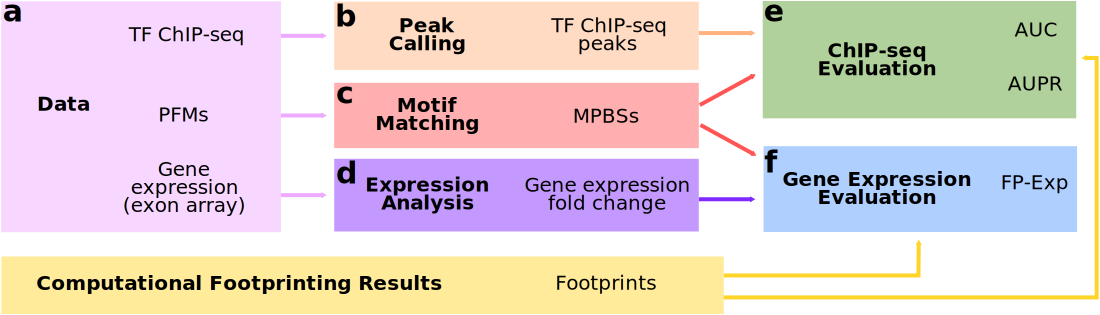
\includegraphics[width=0.99\textwidth]{gusmao_experiment_design_evaluation}
\caption[Experimental framework of the evaluation of the computational footprinting methods]{\textbf{Experimental framework of the evaluation of the computational footprinting methods.} (\textbf{a}) The evaluation methodologies use transcription factor (TF) ChIP-seq, position frequency matrices (PFMs) and gene expression data. (\textbf{b}) A peak calling algorithm is applied to the TF ChIP-seq data to find TF ChIP-seq peaks (enriched regions). (\textbf{c}) The motif matching algorithm is performed using the PFMs to generate motif-predicted binding sites (MPBSs). (\textbf{d}) An expression analysis is performed on the gene expression data to find gene expression fold chance between pairs of cell types. (\textbf{e}) The ChIP-seq evaluation methodology uses MPBSs and TF ChIP-seq peaks as the ground truth. When combined with the footprint predictions, we are able to calculate statistics such as the area under the receiver operating characteristic (ROC) curve (termed AUC) and area under the precision-recall (PR) curve (termed AUPR). (\textbf{f}) The gene expression evaluation methodology uses MPBSs and gene expression fold change (FC) as ground truth. When combined with the footprint predictions, we are able to calculate the FP-Exp statistics (defined in Section~\ref{sec:gene.expression.evaluation}).}
\label{fig:gusmao_experiment_design_evaluation}
\end{figure}

%%%%%%%%%%%%%%%%%%%%%%%%%%%%%%%%%%%%%%%%%%%%%%%%%%%%%%%%%%%%%%%%%%%%%
% Section: Motif-Predicted Binding Sites
%%%%%%%%%%%%%%%%%%%%%%%%%%%%%%%%%%%%%%%%%%%%%%%%%%%%%%%%%%%%%%%%%%%%%
\subsection{Motif-Predicted Binding Sites}
\label{sec:motif.predicted.binding.sites}

% Introduction
MPBSs are predictions of TFBSs made using only the genomic DNA sequence and the proteins' DNA sequence binding affinity. MPBSs are obtained applying a computational sequence-based method. In this thesis we use an algorithm termed motif matching. The motif matching algorithm takes as input the TF DNA sequence binding affinity, represented as a PFM (Figure~\ref{fig:wasserman_pwm}). First, the PFM is normalized, generating another structure called position weight matrix (PWM). Then, the genomic DNA sequence is scanned using the PWM to find substrings which are likely to represent binding sites, given the PWM model. The putative binding sites obtained with the motif matching algorithm are termed MPBSs.

% Section: Data
\subsubsection{Input Data -- Position Frequency Matrix}

% PFMs
PFMs are created by gathering experimentally verified biological sequences which are known to be bound by the target TF of interest. Then, a multiple alignment algorithm is applied to these experimentally verified DNA sequences. After that, conserved positions within this multiple alignment are determined and a specific window, that varies from $5$--$25$ bp is estimated to be the start and end position of the binding affinity representation (Figure~\ref{fig:wasserman_pwm}a and~b). At this point, the PFM $\mathbf{X}^{4 \times m}$ (Figure~\ref{fig:wasserman_pwm}c) is calculated in the following way: each matrix row $i \in D$ with $D = \{\text{A},\text{C},\text{G},\text{T}\}$, correspond to each one of the possible four DNA nucleotides; and the each matrix column $ j \in \{1, \cdots, m\} $ correspond to a position within the motif in the multiple aligned DNA sequences. Consequently, $m$ represents the total length of the motif. Each entry $x_{ij}$ of the PFM corresponds to the number of nucleotides of type $ i $ in position $ j $ of the DNA fragments' multiple alignment.

% Repositories
We obtained all PFMs used on our experiments from the repositories Jaspar~\citep{mathelier2014}, Uniprobe~\citep{robasky2011} and Transfac~\citep{matys2006}. Each TF has its own PFM representation. These non-organism-specific data were obtained for the subphylum \emph{Vertebrata}. See Supplementary Tables~\ref{tab:dataencode.pfm.chipseq} and~\ref{tab:dataencode.pfm.flrexp} for a full description on the PFMs used in this work.

% Section - Position Weight Matrices
\subsubsection{Position Weight Matrices}

% PWMs
From PFMs, we are able to create normalized logarithmic representations termed PWMs $\mathbf{W}^{4 \times m}$ (Figure~\ref{fig:wasserman_pwm}d). The most common method to create PWMs consists on the calculation of the corrected probability $ p_{ij} $ of finding the nucleotide $ i $ in the position $ j $, which is given by
\begin{equation}
  \label{eq:pwm1}
  p_{ij} = \frac{ f_{ij} + s(i) }{ m + {\sum\limits _{i^\prime \in D}{ \hspace{-0.0cm} s(i^\prime)}} }, 
\end{equation}
where $ f_{ij} $ is the frequency of base $ i $ at position $ j $ and $ s(i) $ is a pseudocount function. Pseudocounts are small values used to avoid null probabilities. After the evaluation of the corrected probabilities, the entries $ w_{ij} $ of the PWM are calculated as
\begin{equation}
  \label{eq:pwm2}
  w_{ij} = \log_2 \frac{ p_{ij} }{ b(i) }, 
\end{equation}
where $ b(i) $ is the genomic frequency of nucleotide $ i $ in the genome. The background correction function $b(\cdot)$ is used to correct the PWM for biases regarding the genomic imbalance between the frequencies of the nucleotides.

% Scoring
PWMs are used to score any DNA sequence of length $m$ by a summation of the corresponding nucleotides between the DNA sequence and the PWM (Figure~\ref{fig:wasserman_pwm}e). Such a score is called the PWM's bit-score.

% Information content
Furthermore, we are able to assess the information content $ \mathbf{l} = \langle{l}_{1}, ..., {l}_{m}\rangle $ of each position $ j $ of the PWM $ \mathbf{W} $ by applying
\begin{equation}
  \label{eq:pwm.ic}
  {l}_{j} = 2 + \sum\limits _{i \in D} p_{ij} \log_{2} p_{ij},
\end{equation}
where the number $2$ is obtained from the total possible information content of the $4$-character alphabet $D$, i.e. $\log_{2}4 = 2$. Based on the total information content for every position of the PWM, we are able to create graphical representations of the binding affinity -- termed logo graphs (Figure~\ref{fig:wasserman_pwm}f) -- by multiplying the corrected probability of a certain nucleotide $i$ at a certain position of the PWM $j$ by the total information content at that position (${l}_{j}$).

% Figure - PFMs and PWMs used in the motif matching technique
\begin{figure}[h!]
\centering
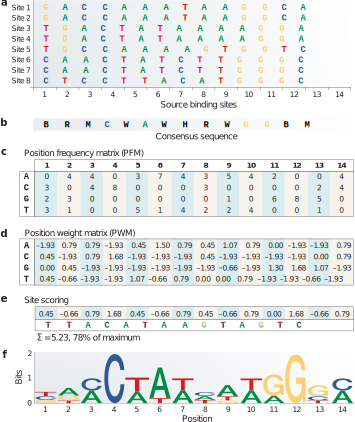
\includegraphics[width=0.92\textwidth]{wasserman_6_pwm}
\caption[PFMs and PWMs used in the motif matching technique]{\textbf{PFMs and PWMs used in the motif matching technique.} (\textbf{a}) A set of experimentally validated binding sites was collected and aligned. The sequence variability of the collection of binding sites strongly affects the downstream models for predicting additional sites. Note the diversity between the sites; for instance, only $50\%$ of the nucleotides are identical between sites one and eight. (\textbf{b}) The consensus sequence model using IUPAC symbols. For instance, the symbol ``B'' means preference for either nucleotides C, G or T. (\textbf{c}) PFMs created based on the source binding sites. (\textbf{d}) PWMs created using the procedure described by Equations~\ref{eq:pwm1} and~\ref{eq:pwm2}. (\textbf{e}) Using the PWM, a quantitative score for any DNA sequence is generated by summing the values that correspond to the observed nucleotide at each position. (\textbf{f}) A sequence logo scales each nucleotide by the total bits of information multiplied by the relative occurrence of the nucleotide at the position (Equation~\ref{eq:pwm.ic}). Sequence logos enable fast and intuitive visual assessment of pattern characteristics. \emph{Source:~\cite{wasserman2004}} (modified to fit thesis format and/or clarify key points).}
\label{fig:wasserman_pwm}
\end{figure}

% Section - Motif Matching
\subsubsection{Motif Matching}

% Motif matching
From a PWM it is possible to estimate the sequence-based probability of the particular TF of binding in the genome. We call this procedure motif matching. For each sequence of nucleotides of length $ m $, a bit-score is calculated. There are also many strategies to perform this calculation. The simplest one is the summation of all the entries in $ w_{ij} $ matching the nucleotide sequence of length $ m $. More formally, given a sequence of characters $\mathbf{g}$ representing the genome, where $\mathbf{g} = \langle{g}_{1}, ..., {g}_{n}\rangle \forall {g}_{i} \in D$. We are able to define a vector of bit-scores $\mathbf{y} = \langle{y}_{1}, ..., {y}_{n-m}\rangle$ as
\begin{equation}
  \label{eq:motif.match}
  {y}_{i} = \sum_{j=1}^{m} \sum_{k \in D} {\mathbf{1}}(k={g}_{i}){w}_{kj},
\end{equation}
where ${\mathbf{1}}(\cdot)$ is an indicator function. 

% Motif match cutoff threshold
A genome-wide application of a PWM creates bit-scores for every possible contiguous nucleotide sequence of length $ N $ within the genome. Then, several statistical techniques can be used to determine a cutoff threshold to accept particular sequences as being bound by the protein, given the PWM. A well-known statistical procedure is to estimate a bit-score cutoff that corresponds to the false positive rate (FPR) of the distribution of the bit-scores from all possible $m$-mers~\citep{wilczynski2009}. More formally, let $C = \{\mathbf{c}^{1}, ..., \mathbf{c}^{4^m}\}$ be the set of all $m$-mers constructed by picking $ m $ elements from the set $ D $ with order and repetition, where each $m$-mer $\mathbf{c}^{i} = \langle{c}^{i}_{1}, \cdots, {c}^{i}_{m}\rangle$. Therefore, we are able to calculate the set $ B = \{ {b}_{1}, \cdots, {b}_{4^m} \} $ of all the possible bit-scores for the PWM $\mathbf{W}$ as
\begin{equation}
  \label{eq:pwm.cutoff1}
  {b}_{i} = \sum_{j=1}^{m} \sum_{k \in D} {\mathbf{1}}(k={c}^{i}_{j}){w}_{kj}.
\end{equation}

% Motif match cutoff threshold
Then, it is easy to find the false discovery rate threshold by finding the $p$-value that corresponds to $ B $ fitted to a certain distribution, say normal
\begin{equation}
  \label{eq:pwm.cutoff2}
  B \sim \mathcal{N}({\mu},{\sigma}^{2}).
\end{equation}

% Set of MPBSs
We observed that the $p$-value choice significantly affects many aspects of the evaluation procedure. Therefore, we made a careful parameter selection analysis. Such an analysis indicated that a $p$-value of $10^{-4}$ resulted in a significant amount of TF ChIP-seq peaks overlapping with MPBSs~\citep{gusmao2014}. Higher $p$-values generate a very high number of MPBSs which impacts on computational time and increases the imbalance between true and false MPBSs~\citep{gusmao2014}. The set of MPBSs after the application of the false discovery rate cutoff threshold is represented by a genomic region set $R = \{ {r}_{1}, \cdots, {r}_{l} \}$, where each MPBS $r_i = [u,v]$, is an interval from genomic positions $u$ to $v$.

%%%%%%%%%%%%%%%%%%%%%%%%%%%%%%%%%%%%%%%%%%%%%%%%%%%%%%%%%%%%%%%%%%%%%
% Section: ChIP-seq Evaluation
%%%%%%%%%%%%%%%%%%%%%%%%%%%%%%%%%%%%%%%%%%%%%%%%%%%%%%%%%%%%%%%%%%%%%
\subsection{ChIP-seq Evaluation}
\label{sec:chipseq.evaluation}

% Introduction
The ChIP-seq evaluation approach uses MPBSs in conjunction with TF ChIP-seq peaks as ground truth~\citep{pique2011,boyle2011,cuellar2012}. By evaluating the overlap between MPBSs, TF ChIP-seq peaks and footprint predictions we are able to assess the accuracy of computational footprinting methods (Figure~\ref{fig:gusmao_chipseq_evaluation_exp}). The advantage of this approach is that it provides a straightforward scenario for the evaluation of computational footprinting methods. Furthermore, this evaluation approach enables the comparison between different methods for each individual TF.

% Section: Data
\subsubsection{Data}

% TF ChIP-seq
We obtained TF ChIP-seq datasets consisting on the enriched regions (peaks). On total, $144$ ChIP-seq peaks datasets were obtained to create the ChIP-seq evaluation datasets. All peaks were obtained in~\cite{encode2012} with exception of the following TFs: (1) AR -- obtained in~\cite{yu2010}; (2) ER -- obtained in~\cite{guertin2014}; and (3) GR -- obtained in~\cite{john2011}. See Supplementary Table~\ref{tab:dataencode.pfm.chipseq} for a full description of TF ChIP-seq data and the TF PFMs matching each ChIP-seq experiment.

% Section: Application of the ChIP-seq Evaluation Methodology
\subsubsection{Application of the ChIP-seq Evaluation Methodology}

% Procedure
MPBSs with ChIP-seq evidence (located within $100$ bp from the ChIP-seq peak summit) are considered ``true'' binding sites; while MPBSs without ChIP-seq evidence are considered ``false'' binding sites. Every TF prediction (footprint) that overlaps a true binding site is considered a correct prediction (true positive -- TP) and every prediction that overlaps a false binding site is considered an incorrect prediction (false positive -- FP). Therefore, true negatives (TN) and false negatives (FN) are, respectively, false and true binding site without overlapping predictions (Figure~\ref{fig:gusmao_chipseq_evaluation_exp}a). We consider overlaps of at least one bp.

% ROC curves and AUC
The contingency table (TPs, FPs, TNs and FNs) enables the creation of receiver operating characteristic (ROC) curves, which describe the sensitivity increase as we decrease the specificity of the method (Figure~\ref{fig:gusmao_chipseq_evaluation_exp}b). The area under the ROC curve (AUC) metric was calculated at $1\%$, $10\%$ and $100\%$ FPRs. By evaluating the AUC at different FPRs we avoid misleading interpretations due to the rate in which the specificity decreases with sensitivity increase. The contingency table also enables the creation of precision-recall (PR) curves (Figure~\ref{fig:gusmao_chipseq_evaluation_exp}c). The area under the PR curve (AUPR) is a statistic indicated for problems with imbalanced datasets (distinct number of positive and negative examples)~\citep{davis2006,fawcett2006}. In summary, the ChIP-seq evaluation methodology provides four performance statistics for each TF: (1) AUC at $1\%$ FPR; (2) AUC at $10\%$ FPR; (3) AUC at $100\%$ FPR; and (4) AUPR. For any of these statistics, higher values indicate higher method performance.

% ChIP-seq evaluation figure
\begin{figure}[h!]
\centering
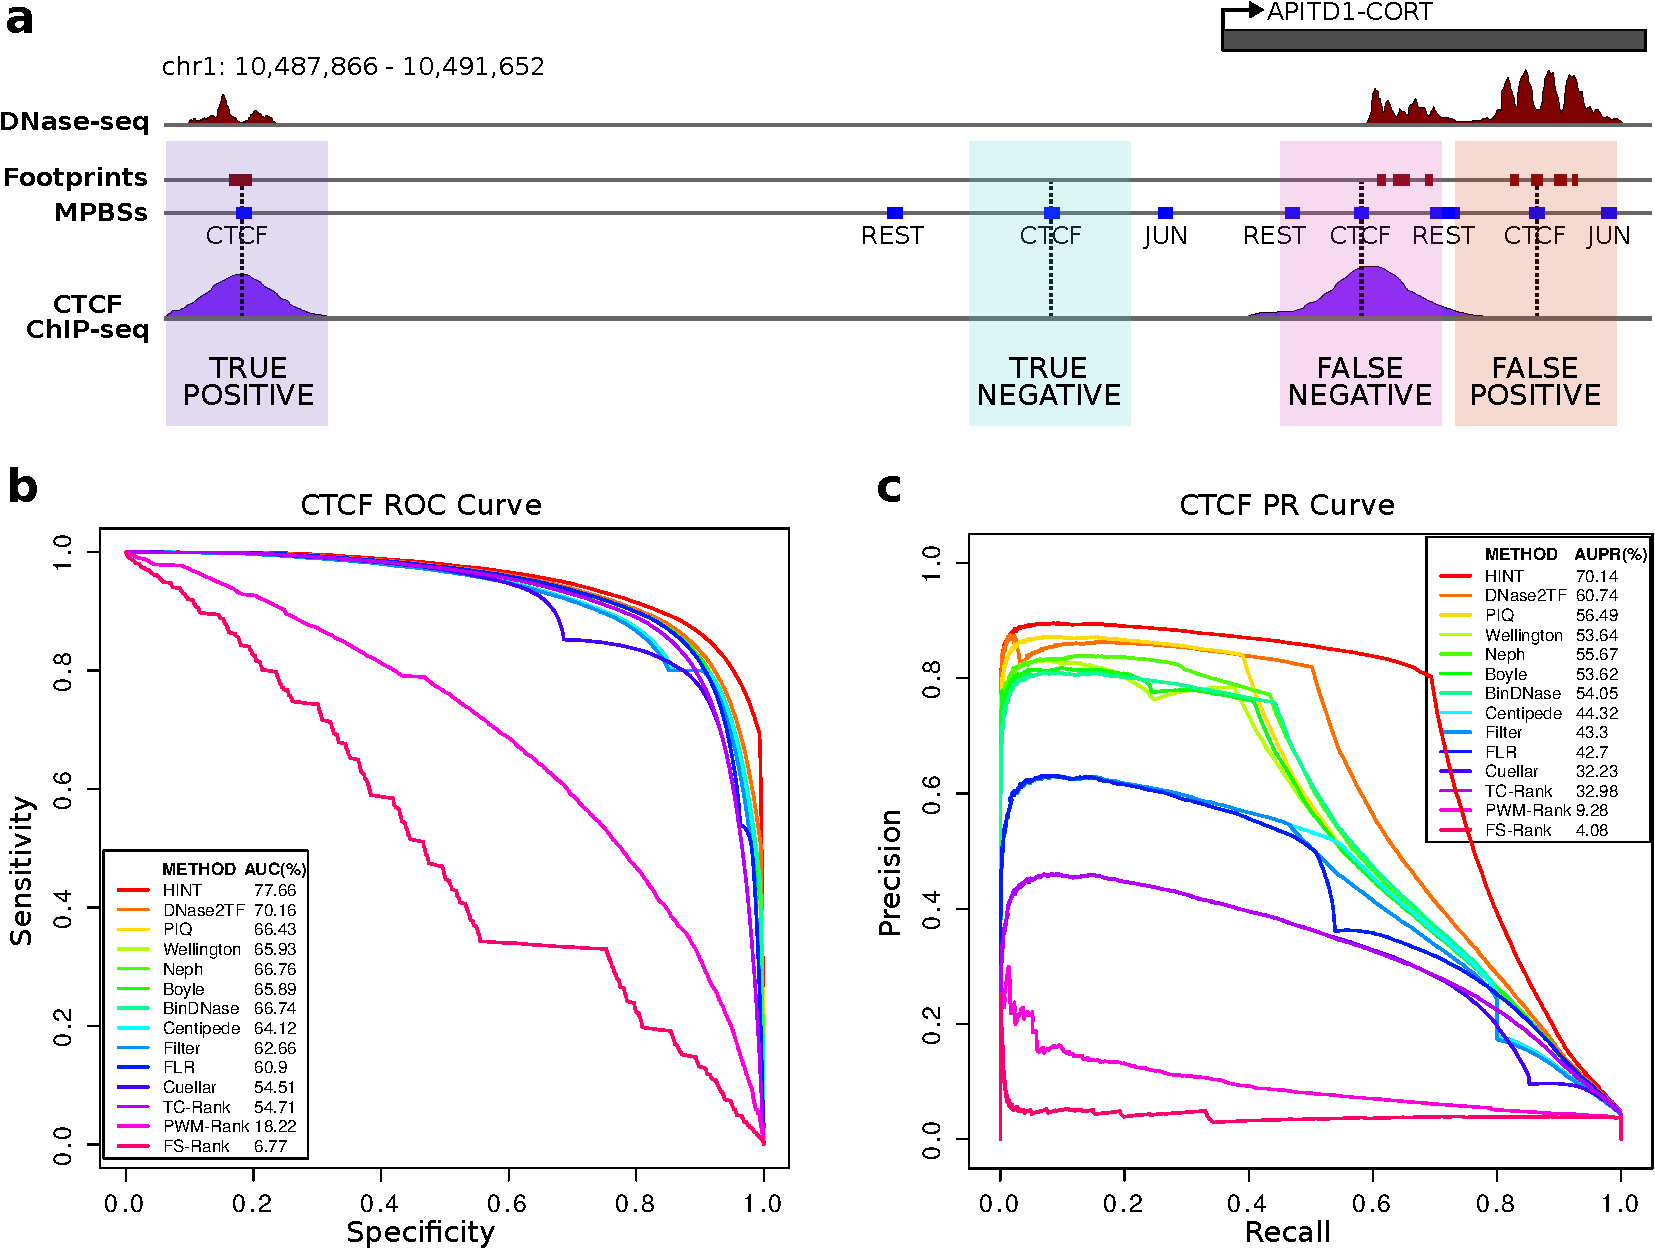
\includegraphics[width=0.99\textwidth]{gusmao_chipseq_evaluation_exp}
\caption[ChIP-seq evaluation methodology]{\textbf{ChIP-seq evaluation methodology.} (\textbf{a}) Example of the ChIP-seq evaluation approach with the real biological data. We are able to calculate a contingency table by checking the overlap between the footprint predictions and the MPBSs with and without cell-specific ChIP-seq evidence. By ranking the MPBSs based on the overlapping footprint's quality, we are able to create: (\textbf{b}) receiver operating characteristic (ROC) curves and (\textbf{c}) precision-recall (PR) curves. These structures can be used to rank the computational footprinting methods and evaluate their overall performance on identifying each TF individually.}
\label{fig:gusmao_chipseq_evaluation_exp}
\end{figure}

% Segmentation full curve and Site-centric threshold
Segmentation-based approaches (Boyle, DNase2TF, HINT, Neph and Wellington) provide footprint predictions that do not necessarily encompass all MPBSs. To create full ROC curves for these methods, we first ranked all predicted sites (MPBS that overlapped a footprint) by their TC (Equation~\ref{eq:tc.exp}) followed all non-predicted sites ranked by their TC. In order to present a fair comparison, this approach was also applied to all site-centric methods (Centipede, Cuellar, FLR and PIQ). For that, we considered distinct probability thresholds of the footprint quality scores reported by each method. We performed additional experiments to select the best threshold per method. We observed that a $p$-value threshold of $0.9$ was best for all site-centric methods except BinDNase, which was best at a $p$-value of $0.8$. These analyses were performed in chromosome-1 which was further removed from the comparative evaluation analyses.

% Section: ChIP-seq Evaluation Scenarios
\subsubsection{ChIP-seq Evaluation Scenarios}

% Evaluation scenarios
Different experiments required a different number of TFs being evaluated. For instance, experiments in which a high number of competing methods were executed, a lower number of TFs were evaluated, given the high demand of computational time. On the other hand, experiments in which a particular computational footprinting feature was being tested using only HINT, we used an evaluation set with a higher number of TFs to enhance statistical significance. Therefore, we created two ChIP-seq evaluation scenarios, described below.

\vspace{0.3cm}

\noindent{{\tt Benchmarking Dataset:}} For comparative analysis of several competing methods, we selected the two cell types from the {\tt Comparative Dataset} (Section~\ref{sec:execution.data}) with the highest number of TF ChIP-seq datasets evaluated in our study: K562 with $59$ TFs and H1-hESC with $29$ TFs. This was required due to the high computational demands of the execution of some competing methods. All methods described in this study were compared under this evaluation scenario (executed using the SH DNase-seq data).

\vspace{0.2cm}

\noindent{{\tt Comprehensive dataset:}} We have compiled a comprehensive dataset containing $235$ combinations of cell types and TFs with matching cellular background. We used the cell types from the {\tt Analysis Dataset} (Section~\ref{sec:execution.data}). This dataset was built from a catalog of $144$ TF ChIP-seq. This dataset was used in analyses which required a large dataset for statistical significance. In this scenario we only evaluated HINT and the baseline methods.

\vspace{0.3cm}

%%%%%%%%%%%%%%%%%%%%%%%%%%%%%%%%%%%%%%%%%%%%%%%%%%%%%%%%%%%%%%%%%%%%%
% Section: Gene Expression Evaluation
%%%%%%%%%%%%%%%%%%%%%%%%%%%%%%%%%%%%%%%%%%%%%%%%%%%%%%%%%%%%%%%%%%%%%
\subsection{Gene Expression Evaluation}
\label{sec:gene.expression.evaluation}

% Introduction
The ChIP-seq evaluation approach requires TF ChIP-seq experiments which, as indicated by~\cite{yardimci2014}, has some intrinsic biases. First, TF ChIP-seq peaks are also observed in indirect binding events. Second, they have a lower spatial resolution than DNase-seq. Therefore, false MPBSs might be regarded as true MPBSs by proximity to an active TFBS. Recently,~\cite{yardimci2014} indicated that footprint quality scores, as measured by their method's metric -- the footprint likelihood ratio (FLR) -- were significantly higher in cells where the TF was expressed. This observation indicates that comparing changes in expression and quality of footprints in a pair of cells provides an alternative footprint evaluation measure. This led us to the development of a novel evaluation methodology based on gene expression by applying this idea systematically for a large set of TFs.

% Section: Data
\subsubsection{Data}

% Gene expression data
Expression profiling by array (Affymetrix Human Exon 1.0 ST Array) data was obtained in~\cite{encode2012}. We obtained data for all {\tt Comparative Dataset} cell types: H1-hESC, K562 and GM12878. All samples from each cell type was used to infer the overall gene expression profile. See Supplementary Table~\ref{tab:data.expression} for a full gene expression data description.

% Section: Application of the Gene Expression Evaluation Methodology
\subsubsection{Application of the Gene Expression Evaluation Methodology}

% Expression
We used limma~\citep{ritchie2015} version 3.28.4 to perform between-array normalization on expression of H1-hESC, K562 and GM12878 cells and obtain gene expression fold change (FC) estimates. This generated pairwise FCs between all three cell type pairs: H1-hESC \emph{vs} K562, H1-hESC \emph{vs} GM12878 and K562 \emph{vs} GM12878. We used the R programming language version 3.1.2 implementation of limma. The source code of this software is found at \url{https://bioconductor.org/packages/release/bioc/html/limma.html}.

% PFMs & MPBSs
Then, we retrieved all non-redundant PFMs from Jaspar in which gene symbol is a perfect match with genes present in the array platform. This leads us to $143$ PFMs (Supplementary Table~\ref{tab:dataencode.pfm.flrexp}). We applied a genome-wide motif matching (Section~\ref{sec:motif.predicted.binding.sites}) using these PFMs to create MPBSs.

% Process
Afterwards, we calculated footprint quality scores for all footprints from all computational footprinting methods, which intersect with MPBSs of a particular motif. In this thesis we used three different metrics as footprint quality scores: (1) the FLR score~\citep{yardimci2014}; (2) the TC and (3) the FS. We only considered the footprints within DHSs that are in common between the cell type pair being evaluated, as described in~\cite{yardimci2014}. We expect that TFs with higher expression values in a particular cell type would present higher values regarding footprint quality metrics with DNase-seq from that cell type.

% Kolmogorov-Smirnov
A two-sample Kolmogorov-Smirnov (KS) test was used to assess the difference between each metrics' distribution between the two cell types being evaluated. The KS statistic, which varies within $[0,1]$, is used to indicate the difference between two distributions; higher values indicate higher differences. As the KS score do not indicate the direction of the changes in distribution, we obtained a signed version by multiplying KS statistic by $-1$, in cases where the median of the quality scores calculated in cell type A $<$ median calculated in cell type B. We calculated the Spearman correlation between the signed KS test statistic and the FC for each TF. Positive values indicate an association between expression of TFs and quality of footprint predictions. We will call this correlation ``FP-Exp''. The higher the FP-Exp, the better the computational footprinting method. Figure~\ref{fig:gusmao_flrexp_evaluation} exhibits a graphical description of the gene expression evaluation methodology.

% FP-Exp evaluation figure
\begin{figure}[h!]
\centering
\vspace{0.8cm}
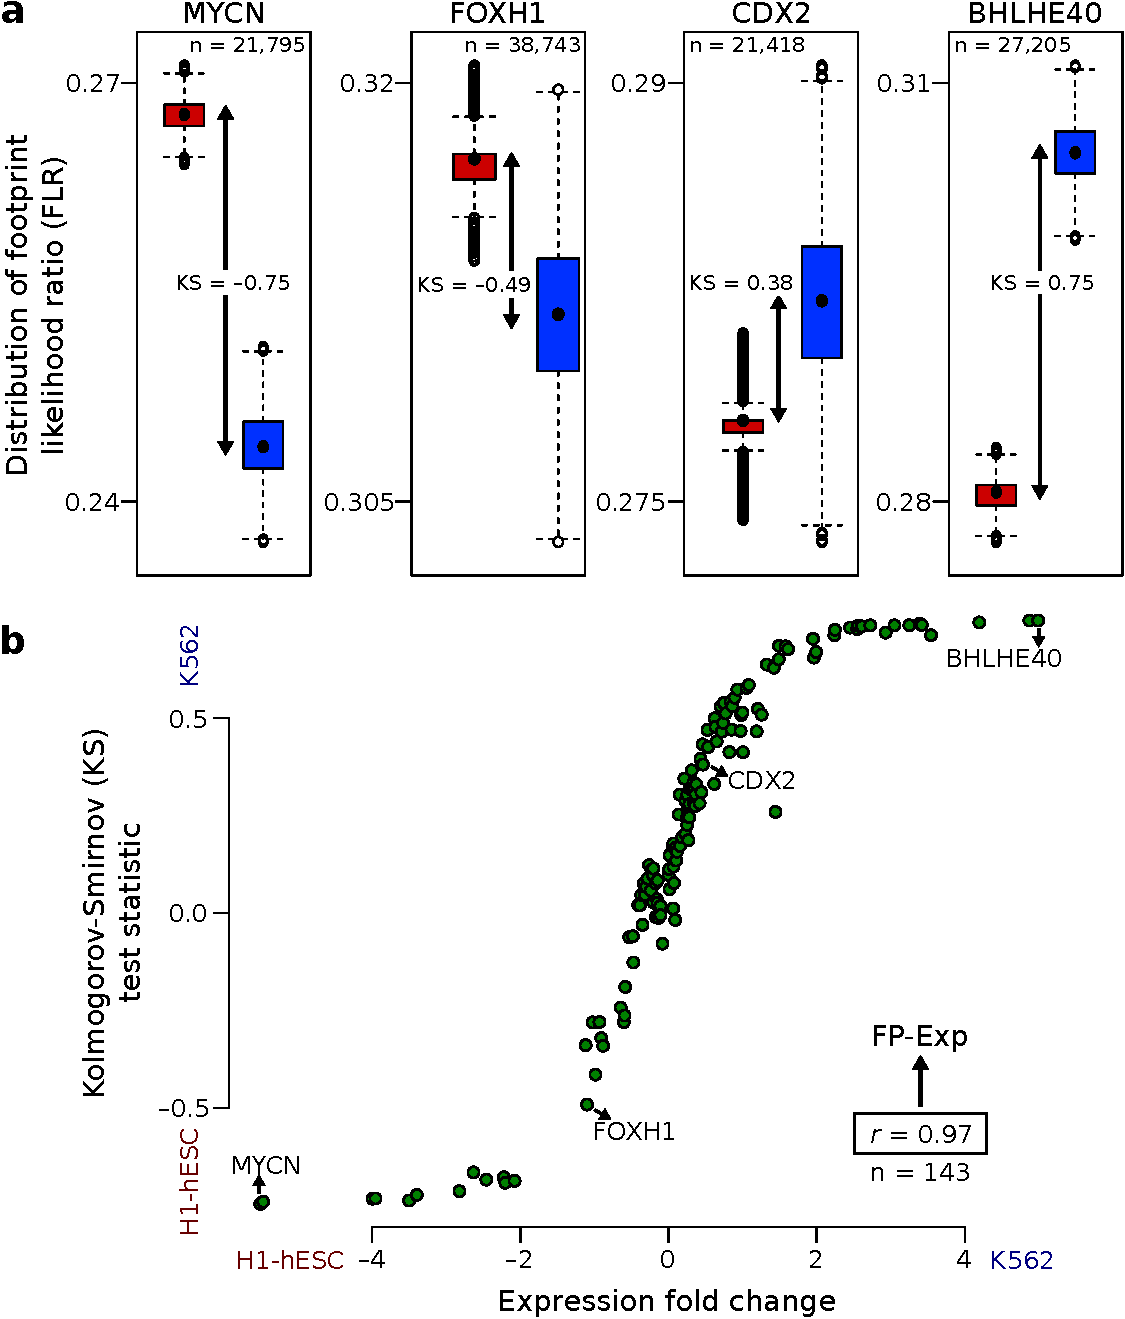
\includegraphics[width=0.86\textwidth]{gusmao_flrexp_evaluation}
\vspace{0.1cm}
\caption[Gene expression evaluation methodology]{\textbf{Gene expression evaluation methodology.} This figure shows an example of the gene expression evaluation methodology using the footprint likelihood ratio (FLR) as a footprint quality score, calculated on DNase-seq data from cell types H1-hESC (SH) and K562 (SH). (\textbf{a}) FLR score distribution of footprints predicted with HINT overlapping with MPBSs of selected TFs. These TFs have increasing expression in K562 (red) compared with H1-hESC cell types (blue). The signed Kolmogorov-Smirnov (KS) statistic quantifies the separation of both distributions. The box plot depicts the distribution median value (middle dot) and first and third quartiles (box extremities). Box plots' whiskers represent the $1.5$ interquartile region (IQR) and external dots represent outliers (data greater than or smaller than $1.5$ IQR). (\textbf{b}) Scatter plot with signed KS statistic and expression fold change (FC) for 143 TFs. There is a clear association between TF expression and KS statistic ($r = 0.97$, adjusted $p$-value $< 10^{-10}$). We call this correlation FP-Exp. The higher the FP-Exp, the better the computational footprinting method. \emph{Source:~\cite{gusmao2016}} (modified to fit thesis format and/or clarify key points).}
\label{fig:gusmao_flrexp_evaluation}
\end{figure}

%%%%%%%%%%%%%%%%%%%%%%%%%%%%%%%%%%%%%%%%%%%%%%%%%%%%%%%%%%%%%%%%%%%%%
% Section: Downstream Analyses
%%%%%%%%%%%%%%%%%%%%%%%%%%%%%%%%%%%%%%%%%%%%%%%%%%%%%%%%%%%%%%%%%%%%%
\section{Downstream Analyses}
\label{sec:footprint.downstream.analyses}

% Introduction
The predicted footprints from a computational footprinting approach represent a map of active TFBSs. In possession of such footprints we are able to perform a number of different downstream analysis. In this section we show two common downstream analyses that we are going to explore in this thesis: the TF enrichment analysis and the \emph{de novo} motif finding. The main goal of the TF enrichment analysis is to identify TFs which are more likely to bind in footprints from a particular cell type when compared to other cell type (Section~\ref{sec:transcription.factor.enrichment.analysis}). On the other hand, the \emph{de novo} motif finding consists on searching for novel TF DNA affinity sequences which do not match any known affinity sequence in the literature (Section~\ref{sec:denovo.motif.finding}).

%%%%%%%%%%%%%%%%%%%%%%%%%%%%%%%%%%%%%%%%%%%%%%%%%%%%%%%%%%%%%%%%%%%%%
% Section: Transcription Factor Enrichment Analysis
%%%%%%%%%%%%%%%%%%%%%%%%%%%%%%%%%%%%%%%%%%%%%%%%%%%%%%%%%%%%%%%%%%%%%
\subsection{Transcription Factor Enrichment Analysis}
\label{sec:transcription.factor.enrichment.analysis}

% Introduction
The TF enrichment analysis is divided in two parts: (1) the application of a statistical test, on each cell type or biological condition, to verify if TFs bind more than expected by chance at genomic regions of interest (i.e. footprints); and (2) the comparison between the results of the statistical test for all TFs between the different cell types or biological conditions being investigated.

% Target vs background genomic region sets
We start by defining two genomic region sets: the target genomic region set and the background genomic region set. The target genomic region set $X = \{ x_1, \cdots, x_n \}$ is composed of the genomic regions associated to the target biological condition being tested (Figure~\ref{fig:gusmao_enrichment_analysis}a). It can be, for instance, footprints identified in a group of differentially expressed genes. The background genomic region set $Y = \{ y_1, \cdots, y_m \}$ (Figure~\ref{fig:gusmao_enrichment_analysis}b) is composed of a collection of random genomic regions throughout the genome. The rationale is that the background genomic region set acts as a ``control'' to which we can compare our target genomic region set against. By comparing the occurrence of putative active TF binding within our target genomic region set $X$ against the background genomic region set $Y$ we can perform a statistical test to assess the enrichment of TFs in $X$. For statistical power, the number of background genomic regions $m$ should be higher than the number of target genomic regions $n$.

% Motif analysis and overlap
After the definition of our target and background genomic region sets, we apply the motif matching algorithm to identify MPBSs within these regions (Figure~\ref{fig:gusmao_enrichment_analysis}c). In the analyses presented in this thesis, the motif matching was performed using all the PFMs available from Jaspar~\citep{mathelier2014} and Uniprobe~\citep{robasky2011}. Then, by overlapping the MPBSs with the target and background genomic region sets, we create the following statistics for each TF $t$ (Figure~\ref{fig:gusmao_enrichment_analysis}d):

\vspace{0.3cm}
\noindent
$a_t$ -- The number of target genomic regions overlapping at least one MPBS from TF $t$. \vspace{0.2cm} \\
$b_t$ -- The number of target genomic regions which do not overlap any MPBS from TF $t$. \vspace{0.2cm} \\
$c_t$ -- The number of background genomic regions overlapping at least one MPBS from TF $t$. \vspace{0.2cm} \\
$d_t$ -- The number of background genomic regions which do not overlap any MPBS from TF $t$.\\
\vspace{0.3cm}

% Fisher's exact test
Then, we apply the Fisher's exact test on the aforementioned statistics $a_t$, $b_t$, $c_t$ and $d_t$. The null hypothesis is defined as: the proportion TF binding at target genomic regions is not greater than the proportion of TF binding at background genomic regions. Nevertheless, since we test a high number of TFs (\approxy$600$ PFMs from Jaspar and Uniprobe) and each one requires a different and independent statistical test, we perform a multiple testing correction. For that, we use the Benjamini and Hochberg method~\citep{benjamini1995} (also known as false discovery rate (FDR) control method). The final result is a list of corrected $p$-values which describes the likelihood of the tested TFs to be associated to the target genomic regions in comparison to the background genomic regions.

% Comparison
In possession of the corrected $p$-value list of TF enrichment for all cell types / biological conditions being tested, we search for the TFs that presented significant $p$-values ($< 0.05$) in particular cell types / biological conditions. For that, we filter the list of TFs for the ones which: (1) present a significant $p$-value in at least one of the conditions tested and (2) present a non significant $p$-value in at least one of the conditions tested. The list of filtered TFs are likely to contain the regulators of specific cell types / biological conditions.

% Figure - TF enrichment analysis
\begin{figure}[h!]
\centering
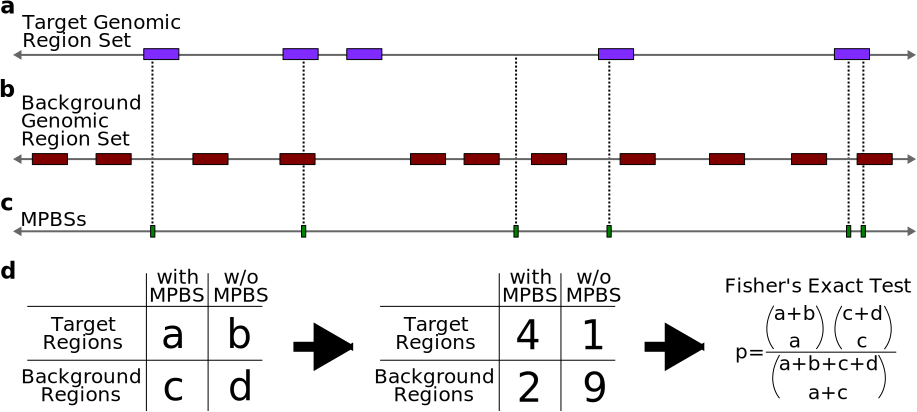
\includegraphics[width=0.99\textwidth]{gusmao_enrichment_analysis}
\caption[TF enrichment analysis]{\textbf{TF enrichment analysis.} (\textbf{a}) The target genomic region set is composed of the genomic regions under study. (\textbf{b}) The background genomic region set is composed of ``control'' genomic regions. It can be, for instance, random genomic regions in the same organism's genome. (\textbf{c}) MPBSs are created for a particular TF in which we are interested in evaluating if it is enriched in the target genomic regions in contrast to the background genomic regions. (\textbf{d}) Based on the overlap between the target genomic region set, the background genomic region set and the MPBSs for a particular TF, we create a contingency table and perform the Fisher's exact test. The test's $p$-value gives an indication on the enrichment of the TF at the target genomic regions.}
\label{fig:gusmao_enrichment_analysis}
\end{figure}

%%%%%%%%%%%%%%%%%%%%%%%%%%%%%%%%%%%%%%%%%%%%%%%%%%%%%%%%%%%%%%%%%%%%%
% Section: De Novo Motif Finding
%%%%%%%%%%%%%%%%%%%%%%%%%%%%%%%%%%%%%%%%%%%%%%%%%%%%%%%%%%%%%%%%%%%%%
\subsection{\emph{De Novo} Motif Finding}
\label{sec:denovo.motif.finding}

% Introduction
We show here a very simple protocol to search for novel TF DNA sequence affinity motifs within footprint predictions. Such analysis extends our knowledge on the regulatory elements that binds a particular cell type.

% Motif matching
First, we apply the motif matching algorithm on all predicted footprints using all PFMs from the Jaspar~\citep{mathelier2014} and Uniprobe~\citep{robasky2011} repositories. Before the motif matching, we extend all footprints by $10$ bp to each side to be able to recognize larger sequence motifs. The goal of this initial motif matching analysis is to eliminate all footprints which correspond to known TF affinity motifs.

% DREME
Then, we apply the \emph{de novo} motif finding tool ``discriminative regular expression motif elicitation'' (DREME)~\citep{bailey2011} on the footprints that do not present any known motif. Such tool is optimized to perform \emph{de novo} motif analysis in datasets containing many sequences and is able to find multiple different motifs. Briefly, DREME finds substrings that appear in a target genomic region set (in our case, the footprints) more frequent than by chance given a background genomic region set (in our case, random genomic regions with the same length of the footprints but with $100$ times more sequences). DREME outputs a number of novel motifs found on the sequence.

% CENTRIMO
Since we performed an extension on the footprints prior to the execution of DREME, we might find a couple of ``artifact motifs'', i.e. small motifs that do not correspond to a footprint which are in the border of the footprint prediction. To filter for these artifact motifs, we execute the ``local motif enrichment analysis'' (CENTRIMO) software~\citep{bailey2012} tool on all sequences associated to the \emph{de novo} motifs found by DREME. This tool makes sure that the motifs found are centrally enriched within the footprints' regions and are not a product of the $10$ bp extension.

% Conclusion
The \emph{de novo} motifs found by DREME which are significantly centrally enriched according to CENTRIMO correspond to the results of our \emph{de novo} motif analyses. These resulting motifs are represented by PFMs based on the DNA sequence on the binding sites within the footprints.

%%%%%%%%%%%%%%%%%%%%%%%%%%%%%%%%%%%%%%%%%%%%%%%%%%%%%%%%%%%%%%%%%%%%%
% Section: Statistical Methods
%%%%%%%%%%%%%%%%%%%%%%%%%%%%%%%%%%%%%%%%%%%%%%%%%%%%%%%%%%%%%%%%%%%%%
\section{Statistical Methods}
\label{sec:further.statistical.methods}

% Comparison between competing methods
All method comparison in this work is performed using the non-parametric Friedman-Nemenyi hypothesis test. This hypothesis test is indicated when using multiple gold standard datasets and methods~\citep{demsar2006}. Such test provides a rank of the methods as well as the statistical significance of whether a particular method was outperformed by other method. The test provides results for the significance levels of $0.95$ and $0.99$. We obtained an implementation of the Friedman-Nemenyi hypothesis test written in Java and it was run in the Java SE Runtime Environment (build 1.8.0\_45-b14).

% Correlation
All correlations calculated in this work are based on the Spearman's rank correlation coefficient (denoted as $r$)~\citep{duda2000}. The Spearman's rank correlation was chosen since it assesses monotonic relationships (whether linear or not). All Spearman correlation $p$-values are based on a two sided test with significance of $0.95$. We used the R programming language version 3.1.2 implementation of the Spearman correlation test with the function \emph{cor.test}.

% Statistical test on diff between two samples
All differences between the distribution of two samples (or more samples in a pair-wise manner) are analyzed using the non-parametric Mann–Whitney–Wilcoxon hypothesis test~\citep{duda2000}. All test $p$-values are based on a two sided test with significance of $0.95$. We used the R programming language version 3.1.2 implementation of the Mann–Whitney–Wilcoxon hypothesis test with the function \emph{wilcox.test}. The only exception is regarding the gene expression evaluation approach (Section~\ref{sec:gene.expression.evaluation}), in which the Kolmogorov-Smirnoff hypothesis test was used, in accordance to~\cite{yardimci2014}.

% Multiple test correction
All $p$-values are corrected for multiple comparisons using the Benjamini and Hochberg method~\citep{benjamini1995} (also known as false discovery rate (FDR) control method). Multiple test correction is necessary since we perform many hypothesis tests given our evaluation framework. We used the R programming language version 3.1.2 implementation of the Benjamini-Hochberg multiple test correction method with the function \emph{p.adjust}.

%%%%%%%%%%%%%%%%%%%%%%%%%%%%%%%%%%%%%%%%%%%%%%%%%%%%%%%%%%%%%%%%%%%%%
% Section: Discussion
%%%%%%%%%%%%%%%%%%%%%%%%%%%%%%%%%%%%%%%%%%%%%%%%%%%%%%%%%%%%%%%%%%%%%
\section{Discussion}
\label{sec:discussion.4}

% Introduction
In this chapter we defined our computational experimental framework. We described the datasets used as input for our computational footprinting method and for the method evaluation experiments. We defined the signal processing, training and execution of our computational footprinting method HINT. Moreover, we described the execution of nine competing methods, categorized as either segmentation-based or site-centric, and four baseline methods, which are regarded as control experiments. In total, our comparative analysis encompasses $14$ different computational footprinting methods. Furthermore, we described the evaluation methodologies, which are based on either TF ChIP-seq or gene expression as ground truth to test footprint predictions. By having two different and independent evaluation approaches we expect to provide a clear picture of the comparison between the tested computational footprinting methods.

% Parameter selection
We have observed that there are a number of parameters from the computational footprinting methods or from the strategies used to generate the evaluation gold standard datasets that have a significant impact on the performance and further analyses results. Therefore, we have performed multiple empirical tests on parameter selection~\citep{gusmao2014}. The parameters shown in this chapter correspond to the ones which maximize the performance of all computational footprinting methods on empirical analyses performed using data from chromosome~1. To avoid overfitting and interpretation biases, we have excluded the chromosome~1 from all our subsequent comparative analyses results. Important results from parameter selection empirical analyses will be shown in the next chapter.

% Novelty
We close this chapter highlighting the main contributions performed in this thesis with regard to the experimental design of computational footprint methods:
\begin{itemize}
\item So far, all studies that perform computational footprinting method comparison used the AUC metric for the ChIP-seq evaluation strategy as a single resource to assess method performance. In this thesis, in addition to using the AUC at various levels of the FPR, we use the AUPR, which is indicated when there is a considerable gold standard data imbalance (very different numbers of positive and negative instances)~\citep{davis2006,fawcett2006}.
\item We devised a novel evaluation strategy which does not rely on ChIP-seq data. Such evaluation strategy uses gene expression fold change from cell type pairs to assess the overall quality of computational footprinting method's performance.
\item No study so far have evaluated such a comprehensive number of different computational footprinting methods. Such a comprehensive analysis provides a full picture of the state-of-the-art strategies for computational footprinting.
\item Finally, we performed multiple parameter selection empirical analyses~\citep{gusmao2014}. Such analyses resulted in maximally efficient footprint predictions for all computational footprinting methods tested, without adding overfitting biases.
\end{itemize}


